\chapter{Methodology}


\section{Introduction}

The Florida iBudget algorithm represents a critical component of the state's developmental disability services infrastructure, determining individual budget allocations for Home and Community-Based Services (HCBS) under the Developmental Disabilities Individual Budgeting waiver program. This system currently serves over 36,000 enrollees, making algorithmic decisions that directly impact the quality of life and service access for individuals with developmental disabilities across Florida. The algorithm's role extends beyond mere budget calculation; it fundamentally shapes how resources are distributed, what services individuals can access, and how person-centered planning principles are implemented in practice.

The enactment of House Bill 1103 in the 2025 legislative session has fundamentally altered the regulatory landscape for iBudget allocation methodologies. This legislation mandates a comprehensive study to review, evaluate, and identify recommendations regarding the current algorithm, with particular emphasis on ensuring compliance with person-centered planning requirements under section 393.0662, Florida Statutes. The bill's requirements extend beyond simple algorithmic refinement, demanding a fundamental reassessment of how statistical methods align with person-centered planning principles and contemporary disability services philosophy.

This analysis addresses three interconnected questions that form the foundation for algorithm evaluation and redesign. 


\section{Technical Architecture and Implementation Framework}

\subsection{System Architecture Overview}

The iBudget model calibration framework implements an object-oriented architecture designed for extensibility, reproducibility, and maintainability. The system employs the Template Method design pattern, where a base abstract class (\texttt{BaseiBudgetModel}) defines the algorithmic skeleton while allowing derived model classes to override specific steps for their unique implementations.

\subsection{Class Hierarchy and Design Patterns}

\subsubsection{Base Abstract Class}

The \texttt{BaseiBudgetModel} abstract class (in \texttt{base\_model.py}) serves as the foundation for all ten alternative models. It enforces a consistent interface while allowing model-specific implementations:

\begin{verbatim}
class BaseiBudgetModel(ABC):
    def __init__(self, model_id: int, model_name: str)
    
    # Abstract methods requiring implementation
    @abstractmethod
    def prepare_features(self, records: List[ConsumerRecord]) 
        -> Tuple[np.ndarray, List[str]]
    
    @abstractmethod
    def fit(self, X: np.ndarray, y: np.ndarray) -> None
    
    @abstractmethod
    def predict(self, X: np.ndarray) -> np.ndarray
    
    # Concrete methods shared across all models
    def load_data(self, cache_file: Path) -> List[ConsumerRecord]
    def split_data(self, test_size: float = 0.2) -> None
    def calculate_metrics(self) -> Dict[str, float]
    def calculate_subgroup_metrics(self) -> Dict[str, Dict[str, float]]
    def perform_cross_validation(self, n_folds: int = 10) 
        -> Dict[str, Any]
    def generate_diagnostic_plots(self) -> None
    def generate_latex_commands(self) -> None
    def save_results(self) -> None
    def run_complete_pipeline(self, fiscal_year_start: int, 
                            fiscal_year_end: int) -> Dict[str, Any]
\end{verbatim}

\subsubsection{Consumer Record Data Structure}

The framework uses a standardized \texttt{ConsumerRecord} dataclass to represent individual client records with comprehensive demographic, clinical, and cost data:

\begin{verbatim}
@dataclass
class ConsumerRecord:
    # Identifiers
    case_no: int
    fiscal_year: int
    
    # Demographics
    age: int
    gender: str
    age_group: str  # Age3_20, Age21_30, Age31Plus
    living_setting: str  # FH, ILSL, RH1-RH4
    county: str
    district: str
    region: str
    
    # Clinical information
    primary_diagnosis: str
    secondary_diagnosis: str
    
    # Cost and utilization
    total_cost: float
    service_days: int
    unique_procedures: int
    unique_providers: int
    
    # QSI Assessment Scores
    bsum: float  # Behavioral sum (Q25-Q30)
    fsum: float  # Functional sum (Q14-Q24)
    psum: float  # Physical sum (Q32-Q50)
    fhfsum: float  # Family Home/Foster sum
    slfsum: float  # Supported Living Functional sum
    slbsum: float  # Supported Living Behavioral sum
    
    # Individual QSI questions (q14-q51a)
    # Data quality flags
    late_entry: bool
    early_exit: bool
    has_multiple_qsi: bool
    usable: bool
\end{verbatim}

\subsubsection{Derived Model Classes}

Each alternative model extends \texttt{BaseiBudgetModel} with specific implementations. The actual model files are:

\begin{itemize}
    \item \textbf{model\_1\_current.py}: Square-root transformation with 9.4\% percentile-based outlier removal
    \item \textbf{model\_2\_gamma.py}: GLM with Gamma family and log link function
    \item \textbf{model\_3\_robust.py}: Huber Regressor for robust regression
    \item \textbf{model\_4\_wls.py}: Weighted Least Squares with heteroscedasticity correction
    \item \textbf{model\_5\_ridge.py}: Ridge regression with cross-validated alpha selection
    \item \textbf{model\_6\_lognormal.py}: Log-normal regression with Duan's smearing retransformation
    \item \textbf{model\_6\_elasticnet.py}: Elastic Net with combined L1/L2 regularization
    \item \textbf{model\_7\_quantile.py}: Quantile regression for median estimation
    \item \textbf{model\_8\_bayesian.py}: Bayesian Ridge for uncertainty quantification
    \item \textbf{model\_9\_random\_forest.py}: Random Forest ensemble method
    \item \textbf{model\_10\_neural.py}: Neural network using Keras/TensorFlow or MLPRegressor
\end{itemize}

\subsection{Directory Structure}

The project follows this actual directory structure:

\begin{verbatim}
iBudget/
├── script/                          # Python code and execution
│   ├── models/
│   │   ├── base_model.py           # Abstract base class
│   │   ├── model_1_current.py      # Current algorithm updated
│   │   ├── model_2_gamma.py        # GLM Gamma
│   │   ├── model_3_robust.py       # Robust regression
│   │   ├── model_4_wls.py          # Weighted least squares
│   │   ├── model_5_ridge.py        # Ridge regression
│   │   ├── model_6_lognormal.py    # Log-normal
│   │   ├── model_6_elasticnet.py   # Elastic Net
│   │   ├── model_7_quantile.py     # Quantile regression
│   │   ├── model_8_bayesian.py     # Bayesian Ridge
│   │   ├── model_9_random_forest.py # Random Forest
│   │   └── model_10_neural.py      # Neural Network
│   ├── APDSampleImport.py          # Sample data import
│   ├── CacheCreation.py            # Pickle cache generation
│   ├── CacheSummary.py             # Cache data inspection
│   ├── FeatureSelection.py         # Feature importance analysis
│   ├── outliers.py                 # Outlier detection analysis
│   ├── ProrationAnalysis.py        # Monthly cost distribution analysis
│   ├── metadata.py                 # Data dictionary generation
│   ├── Model5bRecalibration.py     # Final model recalibration
│   └── Model5bRecalibratedExecution.py  # Production execution
├── report/                          # LaTeX and output files
│   ├── iBudgetReport.tex           # Main document
│   ├── 0.1.config.tex              # Document configuration
│   ├── 0.2.FrontMatter.tex         # Title and TOC
│   ├── 1Introduction.tex           # Introduction chapter
│   ├── 2FeatureSelection.tex       # Feature selection chapter
│   ├── 2Methodology.tex            # Methodology chapter
│   ├── 2PreviousAlgorithm.tex      # Historical context
│   ├── 3AlternativeAlgorithms.tex  # Alternative models overview
│   ├── 3Alternative-[1-10]-*.tex   # Individual model chapters
│   ├── 4Implementation.tex         # Implementation chapter
│   ├── 5Appendix.tex               # Appendix with code listings
│   ├── APD_metadata.tex            # Data dictionary
│   ├── data_quality_analysis.tex   # Data quality findings
│   ├── data_quality_commands.tex   # Dynamic statistics
│   ├── proration_analysis.tex      # Proration analysis
│   ├── proration_commands.tex      # Proration statistics
│   ├── figures/                    # Generated plots and visualizations
│   ├── models/                     # Model-specific outputs
│   │   ├── model_1/
│   │   │   ├── model_1_newcommands.tex      # Command definitions
│   │   │   ├── model_1_renewcommands.tex    # Command values
│   │   │   ├── diagnostic_plots.png         # Six-panel diagnostics
│   │   │   ├── predictions.pkl              # Saved predictions
│   │   │   └── metrics.json                 # Performance metrics
│   │   └── [model_2 through model_10 similar structure]
│   └── logs/                       # Execution logs and outputs
│       ├── model_1_log.txt         # Model 1 execution log
│       ├── model_1_current_ascii.py # ASCII version for LaTeX
│       ├── FeatureSelection.txt    # Feature selection output
│       ├── FeatureSelectionCommands.tex # Feature LaTeX commands
│       └── TopFeaturesTable.tex    # Top features table
├── data/                            # Data cache files
│   └── cache_FY[YYYY].pkl          # Pickled consumer records by FY
├── assets/                          # Project documentation
│   ├── DatabaseDDL.txt             # Database schema
│   ├── DataDictionary.txt          # Variable definitions
│   └── ModelingTemplate.txt        # Modeling instructions
└── SQL/                             # SQL scripts and schema
    └── DatabaseDDL.txt             # Database creation scripts
\end{verbatim}

\subsection{Model Execution Workflow}

\subsubsection{Individual Model Execution}

Each model operates as an independent script that can be executed standalone:

\begin{verbatim}
if __name__ == "__main__":
    # Set global random seed for reproducibility
    np.random.seed(42)
    
    # Initialize model with configuration
    model = Model1Current(
        use_fy2024_only=True,
        use_sqrt_transform=True,
        outlier_percentile=0.094
    )
    
    # Run complete pipeline
    results = model.run_complete_pipeline(
        fiscal_year_start=2024,
        fiscal_year_end=2024,
        test_size=0.2,
        perform_cv=True,
        n_cv_folds=10
    )
    
    # Results automatically saved to:
    # - ../../report/models/model_1/
    # - ../../report/logs/model_1_log.txt
\end{verbatim}

\subsubsection{Pipeline Stages}

The \texttt{run\_complete\_pipeline} method orchestrates the following stages:

\begin{enumerate}
    \item \textbf{Data Loading}: Read cached pickle files containing \texttt{ConsumerRecord} objects
    \item \textbf{Data Splitting}: Stratified 80/20 train-test split with fixed random seed
    \item \textbf{Feature Preparation}: Model-specific feature engineering and transformation
    \item \textbf{Model Training}: Fit model on training data
    \item \textbf{Prediction}: Generate predictions for both train and test sets
    \item \textbf{Metric Calculation}: Compute comprehensive performance metrics
    \item \textbf{Subgroup Analysis}: Calculate metrics by demographic groups
    \item \textbf{Cross-Validation}: 10-fold CV for robust performance estimation
    \item \textbf{Diagnostic Plots}: Generate six-panel diagnostic visualization
    \item \textbf{LaTeX Generation}: Create \texttt{newcommands.tex} and \texttt{renewcommands.tex}
    \item \textbf{Results Persistence}: Save predictions, metrics, and logs
\end{enumerate}

\subsection{Data Flow and Caching System}

\subsubsection{Cache Creation Pipeline}

The \texttt{CacheCreation.py} script extracts data from the SQL Server database and creates fiscal year-specific pickle caches:

\begin{verbatim}
# Database connection
conn_string = (
    "DRIVER={ODBC Driver 17 for SQL Server};"
    "SERVER=.;DATABASE=APD;Trusted_Connection=yes"
)

# Execute stored procedure
cursor.execute("EXEC sp_PrepareModelingData")

# Build ConsumerRecord objects
records = []
for row in cursor.fetchall():
    record = ConsumerRecord(
        case_no=row.CaseNo,
        fiscal_year=row.FiscalYear,
        total_cost=parse_currency(row.TotalCost),
        living_setting=row.LivingSetting,
        age_group=row.AgeGroup,
        # ... additional fields
    )
    records.append(record)

# Save to pickle
with open(f'cache_FY{fiscal_year}.pkl', 'wb') as f:
    pickle.dump(records, f)
\end{verbatim}

\subsubsection{Database Integration}

The system interacts with these primary SQL Server database objects:

\begin{itemize}
    \item \textbf{tbl\_Claims\_MMIS}: Service claims with dates, procedures, and paid amounts
    \item \textbf{tbl\_QSIAssessments}: QSI assessment scores and dates
    \item \textbf{tbl\_Consumer}: Consumer demographics and characteristics
    \item \textbf{tbl\_Plans}: Budget plans and allocations
    \item \textbf{tbl\_PlannedServices}: Planned service details
    \item \textbf{tbl\_Model5b\_Predictions}: Production model predictions
    \item \textbf{sp\_PrepareModelingData}: Stored procedure creating customer-fiscal year dataset
\end{itemize}

\subsection{LaTeX Integration System}

\subsubsection{Two-File Command Structure}

Each model generates two LaTeX command files:

\textbf{1. newcommands.tex} - Command definitions (created once):
\begin{verbatim}
% Model 1 Command Definitions
\newcommand{\ModelOneRsqTrain}{\WarningRunPipeline}
\newcommand{\ModelOneRsqTest}{\WarningRunPipeline}
\newcommand{\ModelOneRMSETrain}{\WarningRunPipeline}
\newcommand{\ModelOneRMSETest}{\WarningRunPipeline}
% ... 100+ additional commands
\end{verbatim}

\textbf{2. renewcommands.tex} - Actual values (updated each run):
\begin{verbatim}
% Model 1 Calibrated Values
\renewcommand{\ModelOneRsqTrain}{0.6523}
\renewcommand{\ModelOneRsqTest}{0.6487}
\renewcommand{\ModelOneRMSETrain}{\$14{,}235.67}
\renewcommand{\ModelOneRMSETest}{\$14{,}512.89}
% ... corresponding values
\end{verbatim}

\subsubsection{Command Generation Rules}

The base class automatically generates LaTeX commands following these naming conventions:

\begin{itemize}
    \item \textbf{Model prefix}: \verb|\ModelOne|, \verb|\ModelTwo|, etc. (numbers spelled out)
    \item \textbf{No numeric characters}: Q16 becomes QOneSix, 3\_20 becomes ThreeToTwenty
    \item \textbf{Underscores removed}: age\_group becomes AgeGroup
    \item \textbf{CamelCase}: All command names use CamelCase formatting
\end{itemize}

\subsection{Metric Calculation and Reporting}

\subsubsection{Core Performance Metrics}

The base class calculates comprehensive metrics automatically:

\begin{verbatim}
def calculate_metrics(self) -> Dict[str, float]:
    """Calculate standard regression metrics"""
    return {
        # R-squared metrics
        'r2_train': r2_score(self.y_train, self.train_predictions),
        'r2_test': r2_score(self.y_test, self.test_predictions),
        'adj_r2_train': 1 - (1 - r2_train) * (n_train - 1) / dof,
        'adj_r2_test': 1 - (1 - r2_test) * (n_test - 1) / dof,
        
        # Error metrics
        'rmse_train': sqrt(mean_squared_error(...)),
        'rmse_test': sqrt(mean_squared_error(...)),
        'mae_train': mean_absolute_error(...),
        'mae_test': mean_absolute_error(...),
        'mape_train': mean_absolute_percentage_error(...),
        'mape_test': mean_absolute_percentage_error(...),
        
        # Information criteria
        'aic': n * log(rss/n) + 2*k,
        'bic': n * log(rss/n) + k*log(n),
        
        # Bias metrics
        'bias_train': mean(residuals_train),
        'bias_test': mean(residuals_test)
    }
\end{verbatim}

\subsubsection{Subgroup Analysis}

Metrics are automatically calculated for demographic subgroups:

\begin{itemize}
    \item \textbf{Age groups}: Age3\_20, Age21\_30, Age31Plus
    \item \textbf{Living settings}: FH (Family Home), ILSL (Independent Living), RH1-RH4 (Residential Habilitation levels)
    \item \textbf{Cost quartiles}: Q1\_Low through Q4\_High
\end{itemize}

For each subgroup, the framework computes R², RMSE, bias, and sample size.

\subsection{Diagnostic Visualization}

\subsubsection{Six-Panel Diagnostic Plot}

Each model generates a standardized six-panel diagnostic plot (\texttt{diagnostic\_plots.png}):

\begin{enumerate}
    \item \textbf{Predicted vs Actual (Training)}: Scatter plot with 45-degree reference line and R² annotation
    \item \textbf{Predicted vs Actual (Test)}: Same for test set to assess generalization
    \item \textbf{Residual Plot}: Residuals vs predicted values to check heteroscedasticity
    \item \textbf{Q-Q Plot}: Normal probability plot to assess residual distribution
    \item \textbf{Model-Specific Plot}: Custom visualization (e.g., weight distribution for WLS, regularization path for Ridge)
    \item \textbf{Performance by Group}: Bar chart showing R² across demographic subgroups
\end{enumerate}

\subsection{Quality Assurance and Reproducibility}

\subsubsection{Reproducibility Features}

\begin{enumerate}
    \item \textbf{Fixed random seeds}: Global seed of 42 for all stochastic operations
    \item \textbf{Comprehensive logging}: Detailed execution logs in \texttt{report/logs/model\_X\_log.txt}
    \item \textbf{Results persistence}: All predictions and metrics saved in pickle/JSON format
    \item \textbf{Version control}: Git tracking of all code and configuration
    \item \textbf{ASCII code copies}: LaTeX-safe ASCII versions in \texttt{logs/} for appendix inclusion
\end{enumerate}

\subsubsection{Logging System}

Each model maintains a dedicated log file with structured output:

\begin{verbatim}
2024-09-23 14:23:45 - MODEL 1 - INFO - ===============================
2024-09-23 14:23:45 - MODEL 1 - INFO - Model 1: Current Algorithm Updated
2024-09-23 14:23:45 - MODEL 1 - INFO - ===============================
2024-09-23 14:23:45 - MODEL 1 - INFO - Loading data...
2024-09-23 14:23:46 - MODEL 1 - INFO - Loaded 29,737 records
2024-09-23 14:23:46 - MODEL 1 - INFO - Splitting data (80/20)...
2024-09-23 14:23:46 - MODEL 1 - INFO - Training: 23,789, Test: 5,948
2024-09-23 14:23:46 - MODEL 1 - INFO - Preparing features...
2024-09-23 14:23:47 - MODEL 1 - INFO - Features: 22 columns
...
\end{verbatim}

\subsection{Production Deployment Framework}

\subsubsection{Model 5b Final Implementation}

The selected final model (Model 5b) has dedicated production scripts:

\begin{itemize}
    \item \textbf{Model5bRecalibration.py}: Annual recalibration using updated data
    \item \textbf{Model5bRecalibratedExecution.py}: Batch prediction generation for new assessments
    \item \textbf{Model5bDBVerification.py}: Validation of predictions against database
\end{itemize}

\subsection{Computational Requirements}

\begin{itemize}
    \item \textbf{Hardware}: Minimum 8GB RAM, 4 CPU cores recommended
    \item \textbf{Execution time}: Individual model $<$ 5 minutes on standard hardware
    \item \textbf{Storage}: Approximately 2GB for cache files and outputs per fiscal year
    \item \textbf{Dependencies}: Python 3.9+, scikit-learn 1.0+, statsmodels 0.13+, pandas 1.3+
\end{itemize}

\subsection{Conclusion}

This technical architecture provides a robust, maintainable framework for the iBudget model calibration project. The object-oriented design with the \texttt{BaseiBudgetModel} abstract class ensures code reusability across all seven alternative models. The modular structure with independent model execution facilitates parallel development and testing. The comprehensive LaTeX integration system ensures reproducible reporting with dynamically updated metrics. The pickle-based caching system provides fast data access while maintaining data integrity. This systematic approach enables rigorous comparison of alternative algorithms and evidence-based selection of the optimal model for Florida's disability services budget allocation.


% % Include dynamically generated statistics
% % Automatically generated data quality statistics
% Generated: 2025-09-28 18:18:32

% Overall statistics
\renewcommand{\TheTotalNumberCustomers}{41,285}
\renewcommand{\TheInitialYear}{2019}
\renewcommand{\TheFinalYear}{2024}
\renewcommand{\TheTotalCustomerYears}{212,924}

% Customer data availability
\renewcommand{\CustomerNumberOneYear}{25,347}
\renewcommand{\CustomerPctOneYear}{61.4}
\renewcommand{\CustomerNumberTwoPlusYear}{14,995}
\renewcommand{\CustomerPctTwoPlusYear}{36.3}
\renewcommand{\CustomerNumberNoData}{15,938}
\renewcommand{\CustomerPctNoData}{38.6}

% Exclusion statistics
\renewcommand{\ExclusionMidYearQSICount}{957}
\renewcommand{\ExclusionMidYearQSIPct}{0.5}
\renewcommand{\ExclusionLateEntryCount}{43,102}
\renewcommand{\ExclusionLateEntryPct}{20.2}
\renewcommand{\ExclusionEarlyExitCount}{14,873}
\renewcommand{\ExclusionEarlyExitPct}{7.0}
\renewcommand{\ExclusionNoCostsCount}{109}
\renewcommand{\ExclusionNoCostsPct}{0.1}
\renewcommand{\ExclusionInsufficientServiceCount}{81,901}
\renewcommand{\ExclusionInsufficientServicePct}{38.5}
\renewcommand{\ExclusionNoQSICount}{128,791}
\renewcommand{\ExclusionNoQSIPct}{60.5}

% Cost statistics
\renewcommand{\AvgAnnualCost}{\$33,987}
\renewcommand{\MedianAnnualCost}{\$15,454}
\renewcommand{\StdevAnnualCost}{\$40,545}

% Trajectory analysis
\renewcommand{\CustomersWithTrajectory}{14,995}
\renewcommand{\PctWithTrajectory}{36.3}
\renewcommand{\CustomersWithGaps}{177}
\renewcommand{\PctWithGaps}{0.4}

% Outlier statistics
\renewcommand{\OutlierLowerFence}{\$-153,231}
\renewcommand{\OutlierUpperFence}{\$261,983}
\renewcommand{\OutliersBelow}{0}
\renewcommand{\OutliersAbove}{111}
\renewcommand{\OutlierRate}{0.23}


% \section{Overview}

% This chapter presents the comprehensive methodology for calibrating and evaluating ten alternative models for the Florida iBudget algorithm. The framework addresses significant data quality challenges, implements sophisticated outlier detection strategies, and ensures reproducibility through a unified pipeline architecture. The approach balances statistical rigor with practical constraints imposed by incomplete longitudinal data and irregular service utilization patterns.

% % ⚠ ======================================== ⚠ 
% % ⚠  DO *NOT* EDIT data_quality_commands.tex ⚠ 
% % ⚠  DO *NOT* EDIT data_quality_analysis.tex ⚠ 
% % ⚠ ======================================== ⚠ 
% % These files are produced by executing the program Outliers.py
% % Any change in those files will be lost with every execution of the analysis pipeline 
% % Automatically generated data quality statistics
% Generated: 2025-09-28 18:18:32

% Overall statistics
\renewcommand{\TheTotalNumberCustomers}{41,285}
\renewcommand{\TheInitialYear}{2019}
\renewcommand{\TheFinalYear}{2024}
\renewcommand{\TheTotalCustomerYears}{212,924}

% Customer data availability
\renewcommand{\CustomerNumberOneYear}{25,347}
\renewcommand{\CustomerPctOneYear}{61.4}
\renewcommand{\CustomerNumberTwoPlusYear}{14,995}
\renewcommand{\CustomerPctTwoPlusYear}{36.3}
\renewcommand{\CustomerNumberNoData}{15,938}
\renewcommand{\CustomerPctNoData}{38.6}

% Exclusion statistics
\renewcommand{\ExclusionMidYearQSICount}{957}
\renewcommand{\ExclusionMidYearQSIPct}{0.5}
\renewcommand{\ExclusionLateEntryCount}{43,102}
\renewcommand{\ExclusionLateEntryPct}{20.2}
\renewcommand{\ExclusionEarlyExitCount}{14,873}
\renewcommand{\ExclusionEarlyExitPct}{7.0}
\renewcommand{\ExclusionNoCostsCount}{109}
\renewcommand{\ExclusionNoCostsPct}{0.1}
\renewcommand{\ExclusionInsufficientServiceCount}{81,901}
\renewcommand{\ExclusionInsufficientServicePct}{38.5}
\renewcommand{\ExclusionNoQSICount}{128,791}
\renewcommand{\ExclusionNoQSIPct}{60.5}

% Cost statistics
\renewcommand{\AvgAnnualCost}{\$33,987}
\renewcommand{\MedianAnnualCost}{\$15,454}
\renewcommand{\StdevAnnualCost}{\$40,545}

% Trajectory analysis
\renewcommand{\CustomersWithTrajectory}{14,995}
\renewcommand{\PctWithTrajectory}{36.3}
\renewcommand{\CustomersWithGaps}{177}
\renewcommand{\PctWithGaps}{0.4}

% Outlier statistics
\renewcommand{\OutlierLowerFence}{\$-153,231}
\renewcommand{\OutlierUpperFence}{\$261,983}
\renewcommand{\OutliersBelow}{0}
\renewcommand{\OutliersAbove}{111}
\renewcommand{\OutlierRate}{0.23}

% \section{Data Quality and Outlier Analysis}

\subsection{Overview}

This section presents a comprehensive analysis of data quality and outlier identification for the iBudget model calibration. The analysis examines customer-year records to identify data quality issues and determine the usable dataset for model development.

\subsection{Data Availability Assessment}

The initial data quality analysis examined \TheTotalNumberCustomers{} unique customers in the Agency for Persons with Disabilities (APD) database, spanning fiscal years \TheInitialYear{} through \TheFinalYear{}. Each fiscal year runs from September 1 through August 31, creating potential complications when Questionnaire for Situational Information (QSI) assessments occur mid-year.

The outlier analysis revealed substantial data quality challenges:
\begin{itemize}
    \item \textbf{\CustomerNumberOneYear{} customers (\CustomerPctOneYear\%)} have at least one fiscal year of usable data
    \item \textbf{\CustomerNumberTwoPlusYear{} customers (\CustomerPctTwoPlusYear\%)} have two or more years suitable for trajectory modeling
    \item \textbf{\CustomerNumberNoData{} customers (\CustomerPctNoData\%)} have no usable data after applying quality criteria
\end{itemize}

\subsection{Customer Coverage Analysis}

\begin{figure}[h]
    \centering
    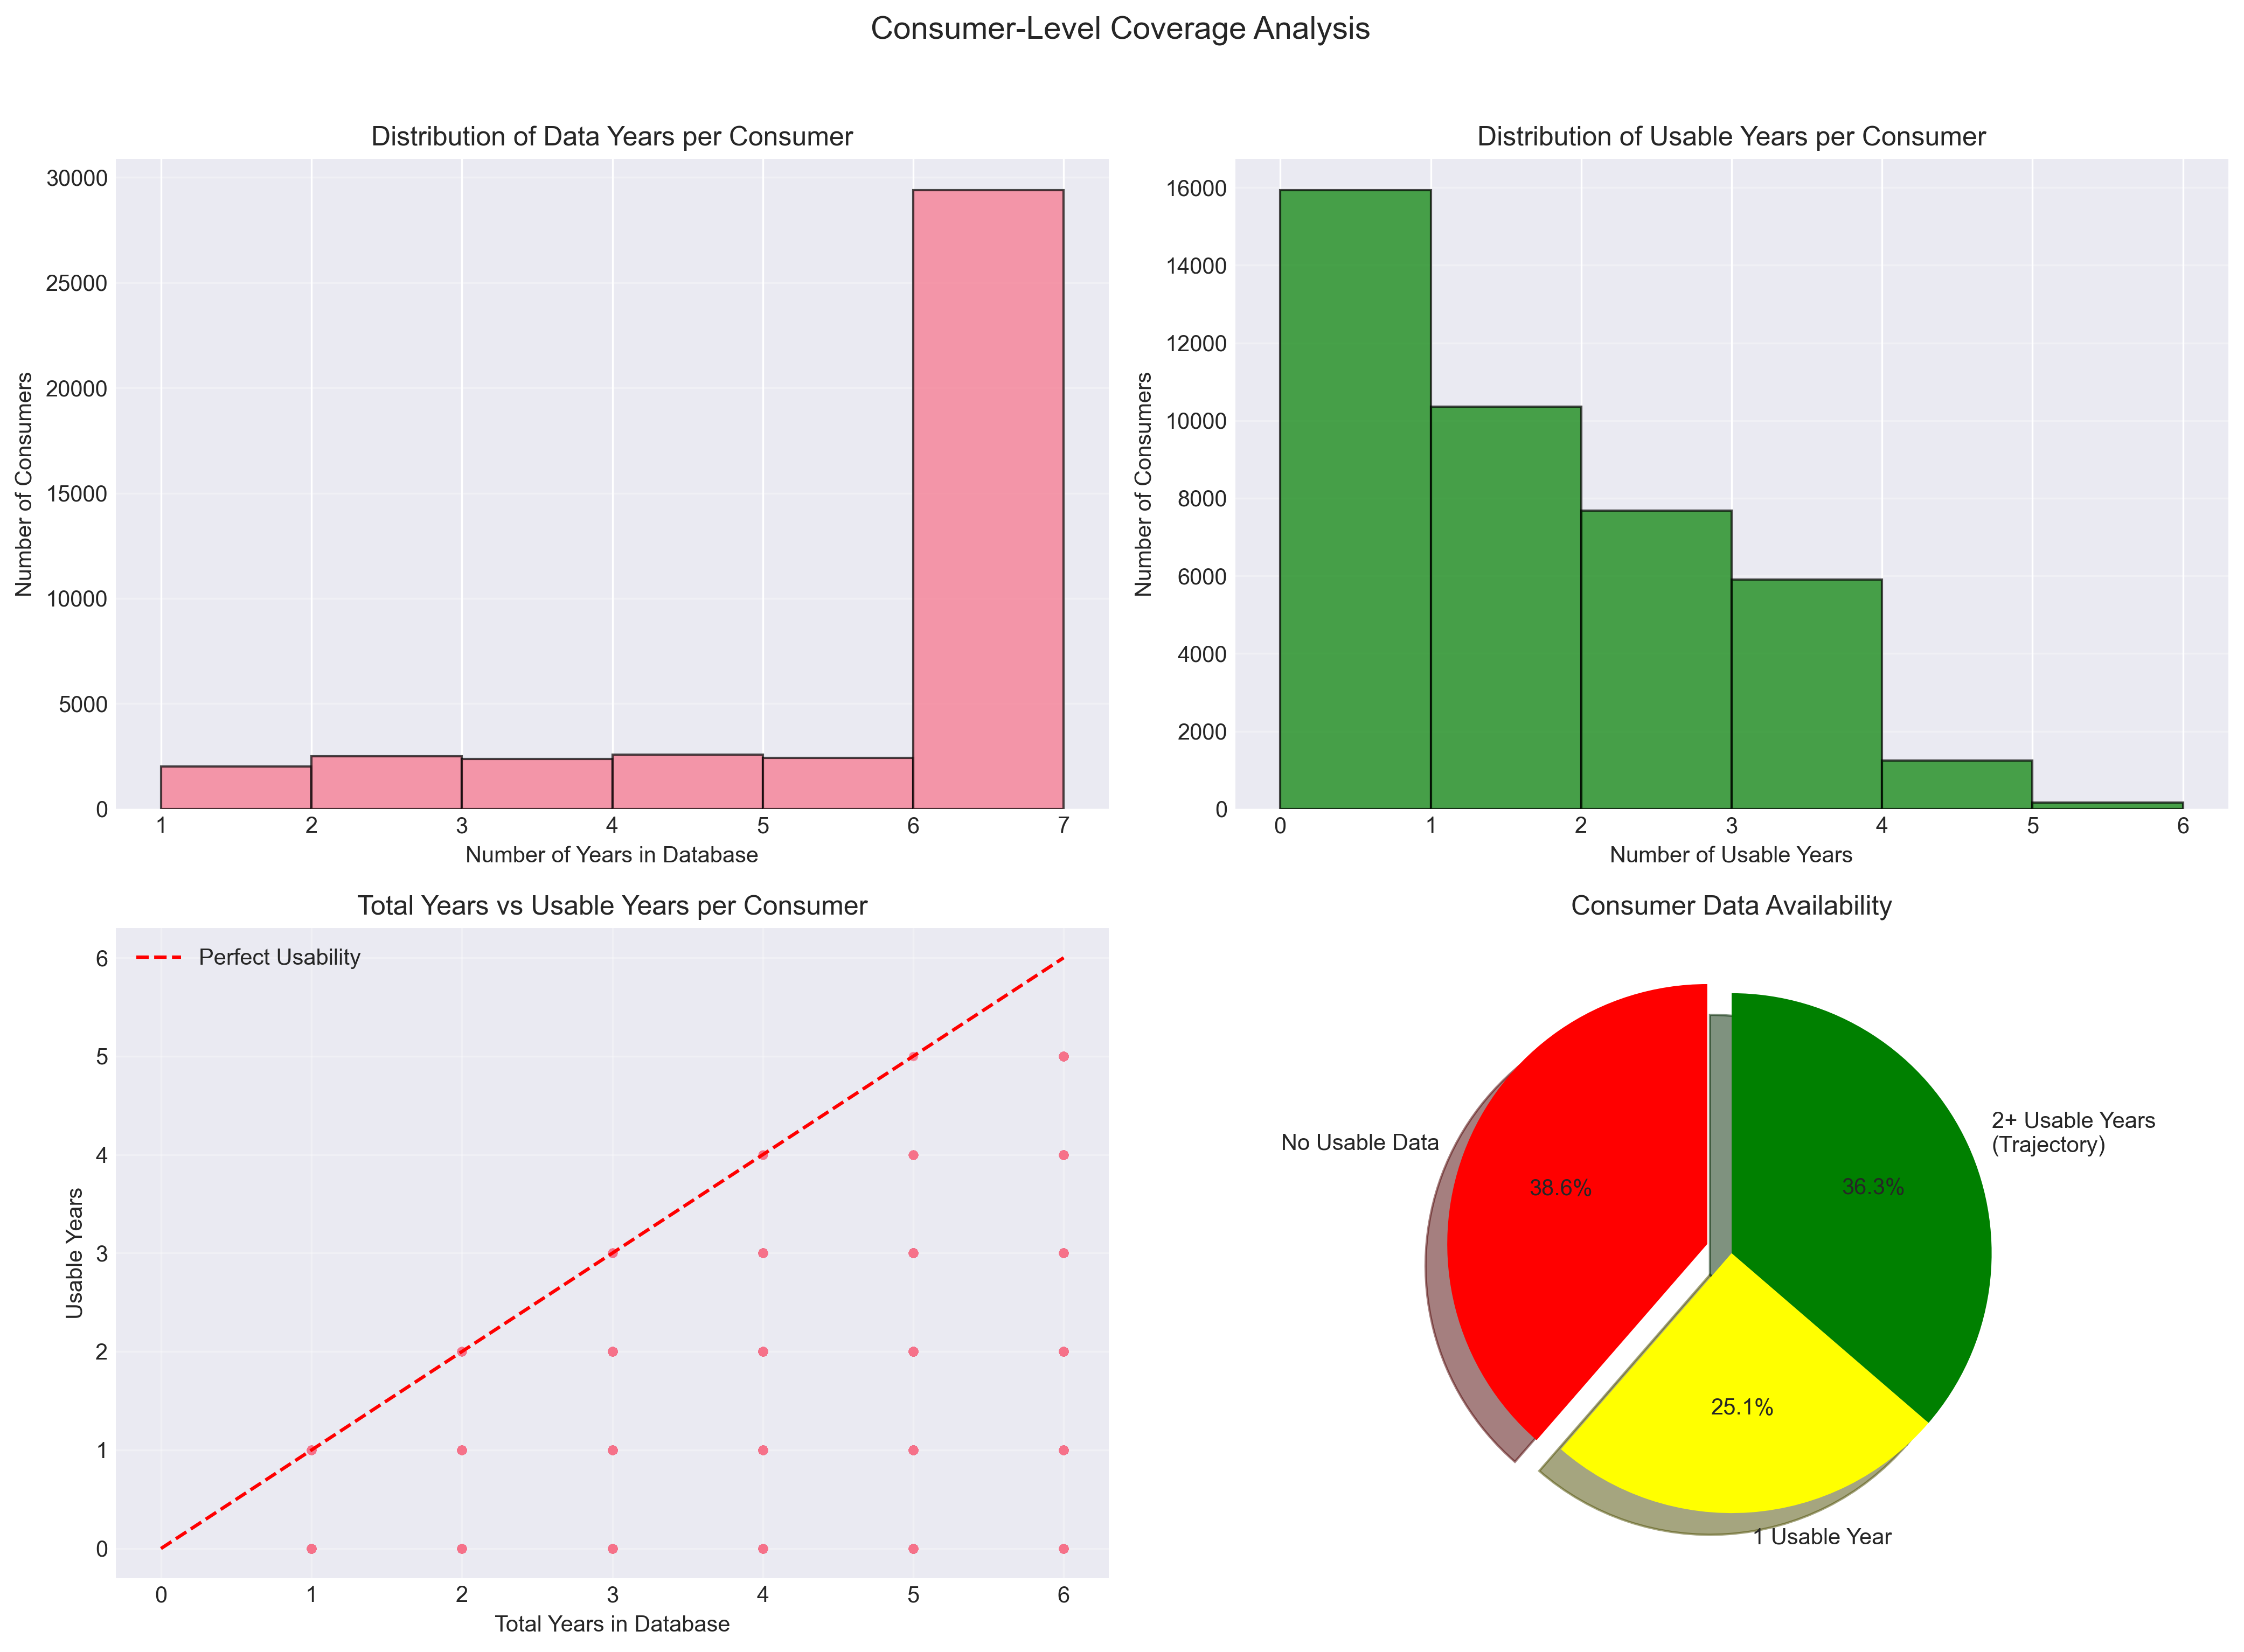
\includegraphics[width=\textwidth]{figures/consumer_coverage.png}
    \caption{Customer-level data coverage analysis}
    \label{fig:customer_coverage}
\end{figure}

Figure~\ref{fig:customer_coverage} presents four panels analyzing customer data availability:
\begin{itemize}
    \item \textbf{Top-left panel}: Distribution of total years each customer appears in the database, showing most customers have either 1-2 years or the full span of data
    \item \textbf{Top-right panel}: Distribution of usable years after applying quality criteria, revealing significant data loss for many customers
    \item \textbf{Bottom-left panel}: Scatter plot comparing total versus usable years, with the red diagonal line representing perfect data usability; points below the line indicate data quality issues
    \item \textbf{Bottom-right panel}: Pie chart showing the critical breakdown---only \CustomerPctTwoPlusYear\% of customers have sufficient data for trajectory modeling
\end{itemize}

\subsection{Data Exclusion Analysis}

Customer-year records are evaluated for several quality issues that would compromise model calibration:

\begin{table}[h]
\centering
\caption{Exclusion Reasons and Impact}
\begin{tabular}{lrr}
\toprule
\textbf{Exclusion Reason} & \textbf{Count} & \textbf{Percentage} \\
\midrule
Mid-Year QSI Change & \ExclusionMidYearQSICount & \ExclusionMidYearQSIPct\% \\
Late Entry (>30 days) & \ExclusionLateEntryCount & \ExclusionLateEntryPct\% \\
Early Exit (>30 days) & \ExclusionEarlyExitCount & \ExclusionEarlyExitPct\% \\
No Costs Recorded & \ExclusionNoCostsCount & \ExclusionNoCostsPct\% \\
Insufficient Service Days & \ExclusionInsufficientServiceCount & \ExclusionInsufficientServicePct\% \\
No QSI Assessment & \ExclusionNoQSICount & \ExclusionNoQSIPct\% \\
\bottomrule
\end{tabular}
\end{table}

\begin{figure}[h]
    \centering
    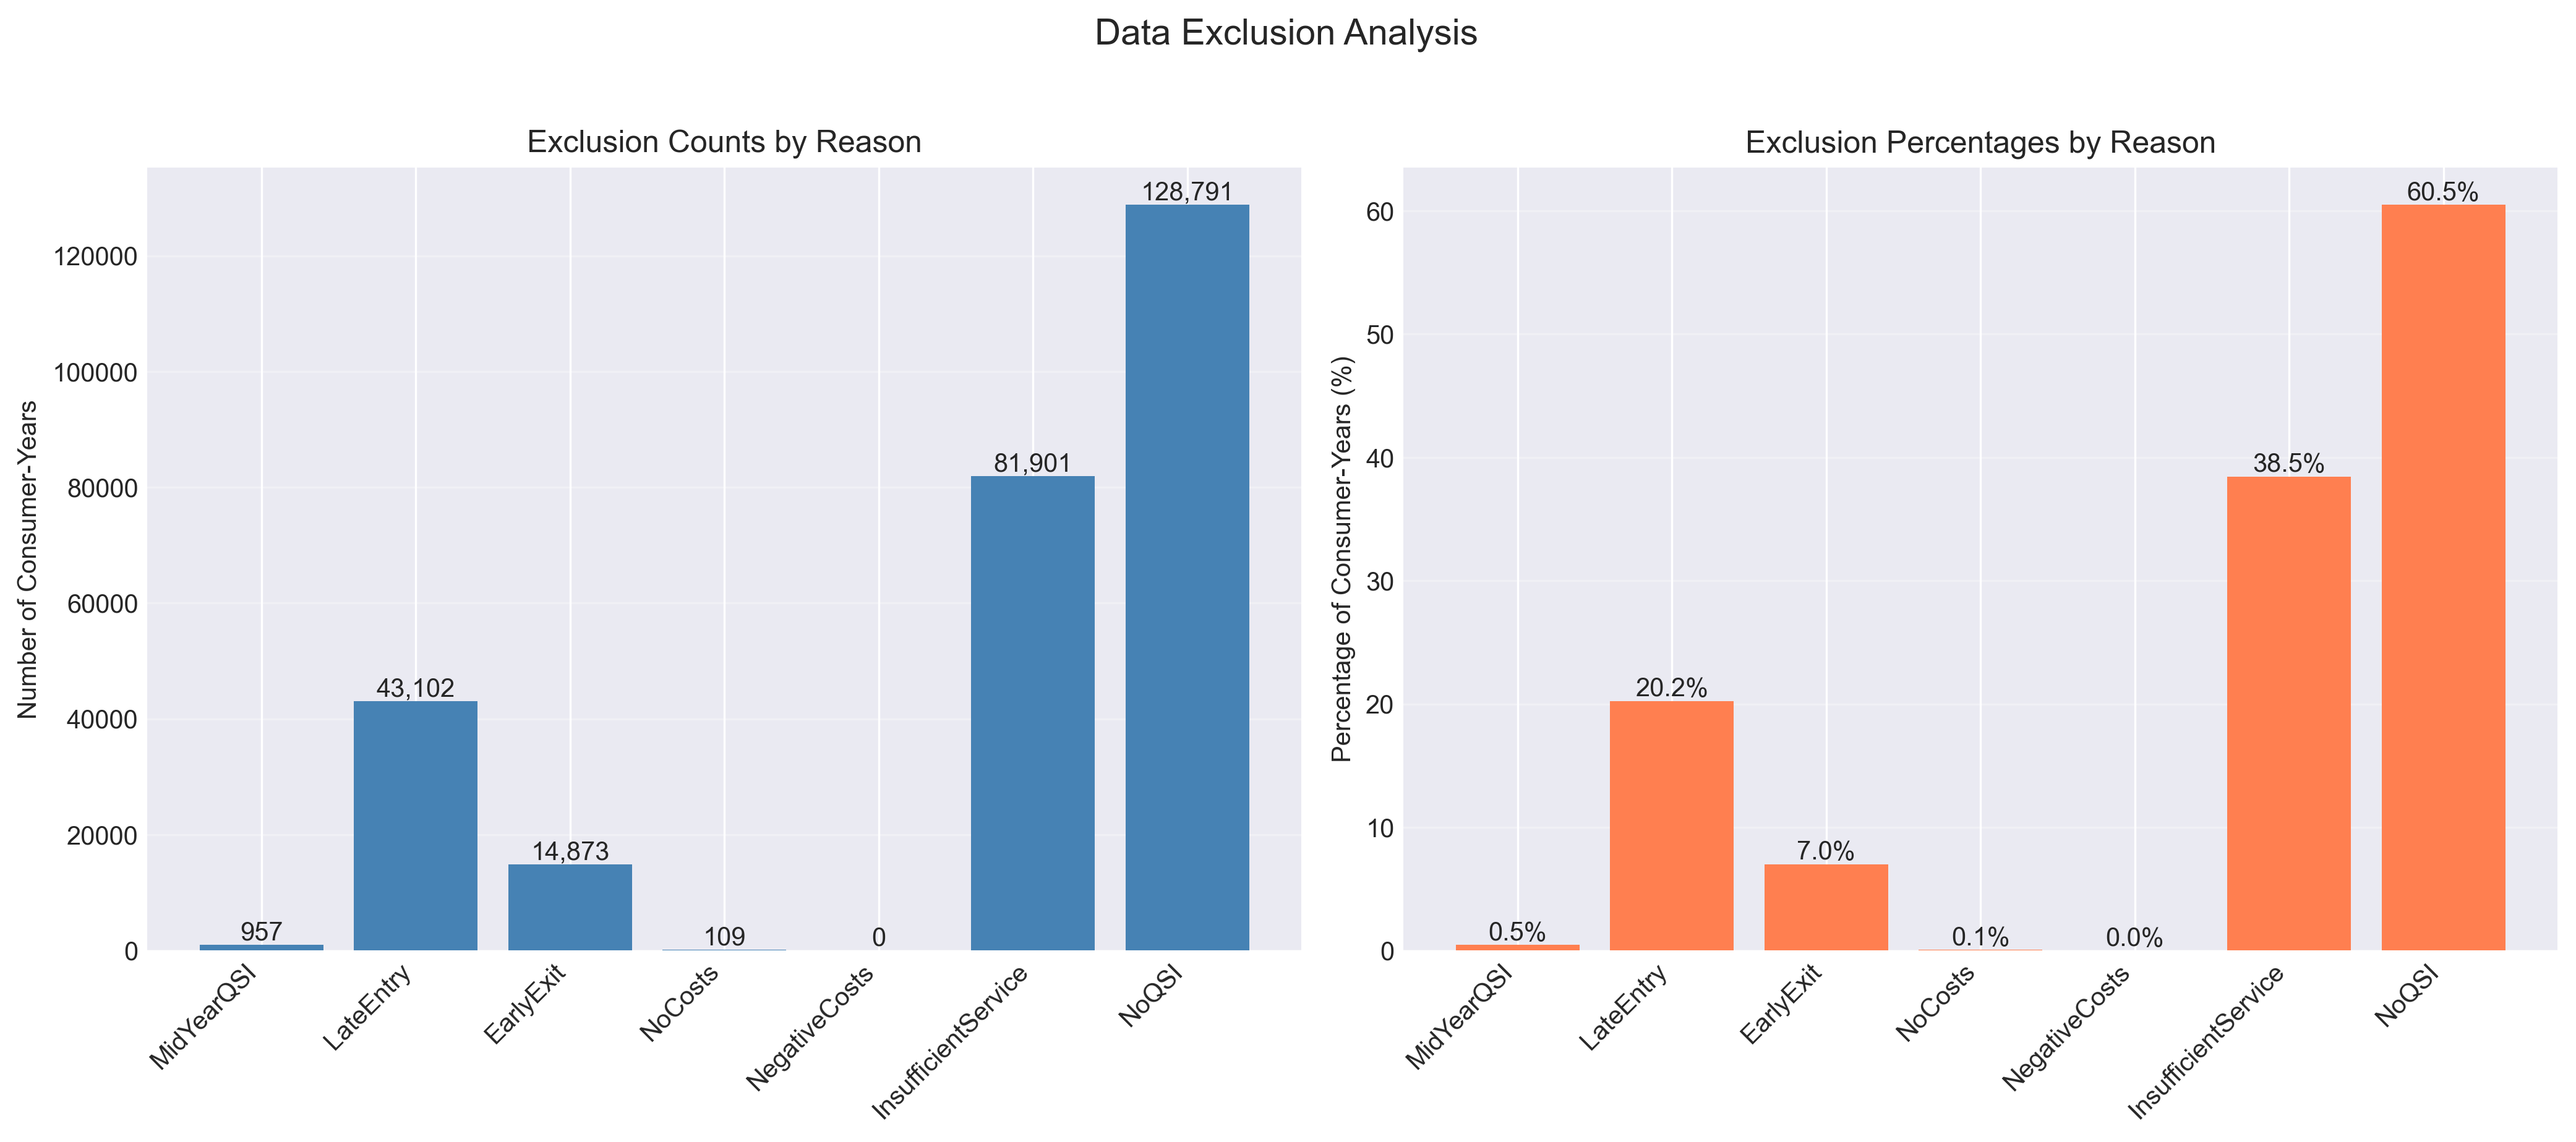
\includegraphics[width=\textwidth]{figures/exclusion_reasons.png}
    \caption{Distribution of exclusion reasons}
    \label{fig:exclusion_reasons}
\end{figure}

Figure~\ref{fig:exclusion_reasons} visualizes the exclusion analysis:
\begin{itemize}
    \item \textbf{Left panel}: Absolute counts of customer-years excluded for each reason, showing the scale of data loss
    \item \textbf{Right panel}: Percentage breakdown highlighting that mid-year QSI changes and incomplete fiscal years are the primary exclusion drivers
\end{itemize}

\subsection{Cost Distribution Analysis}

\begin{figure}[h]
    \centering
    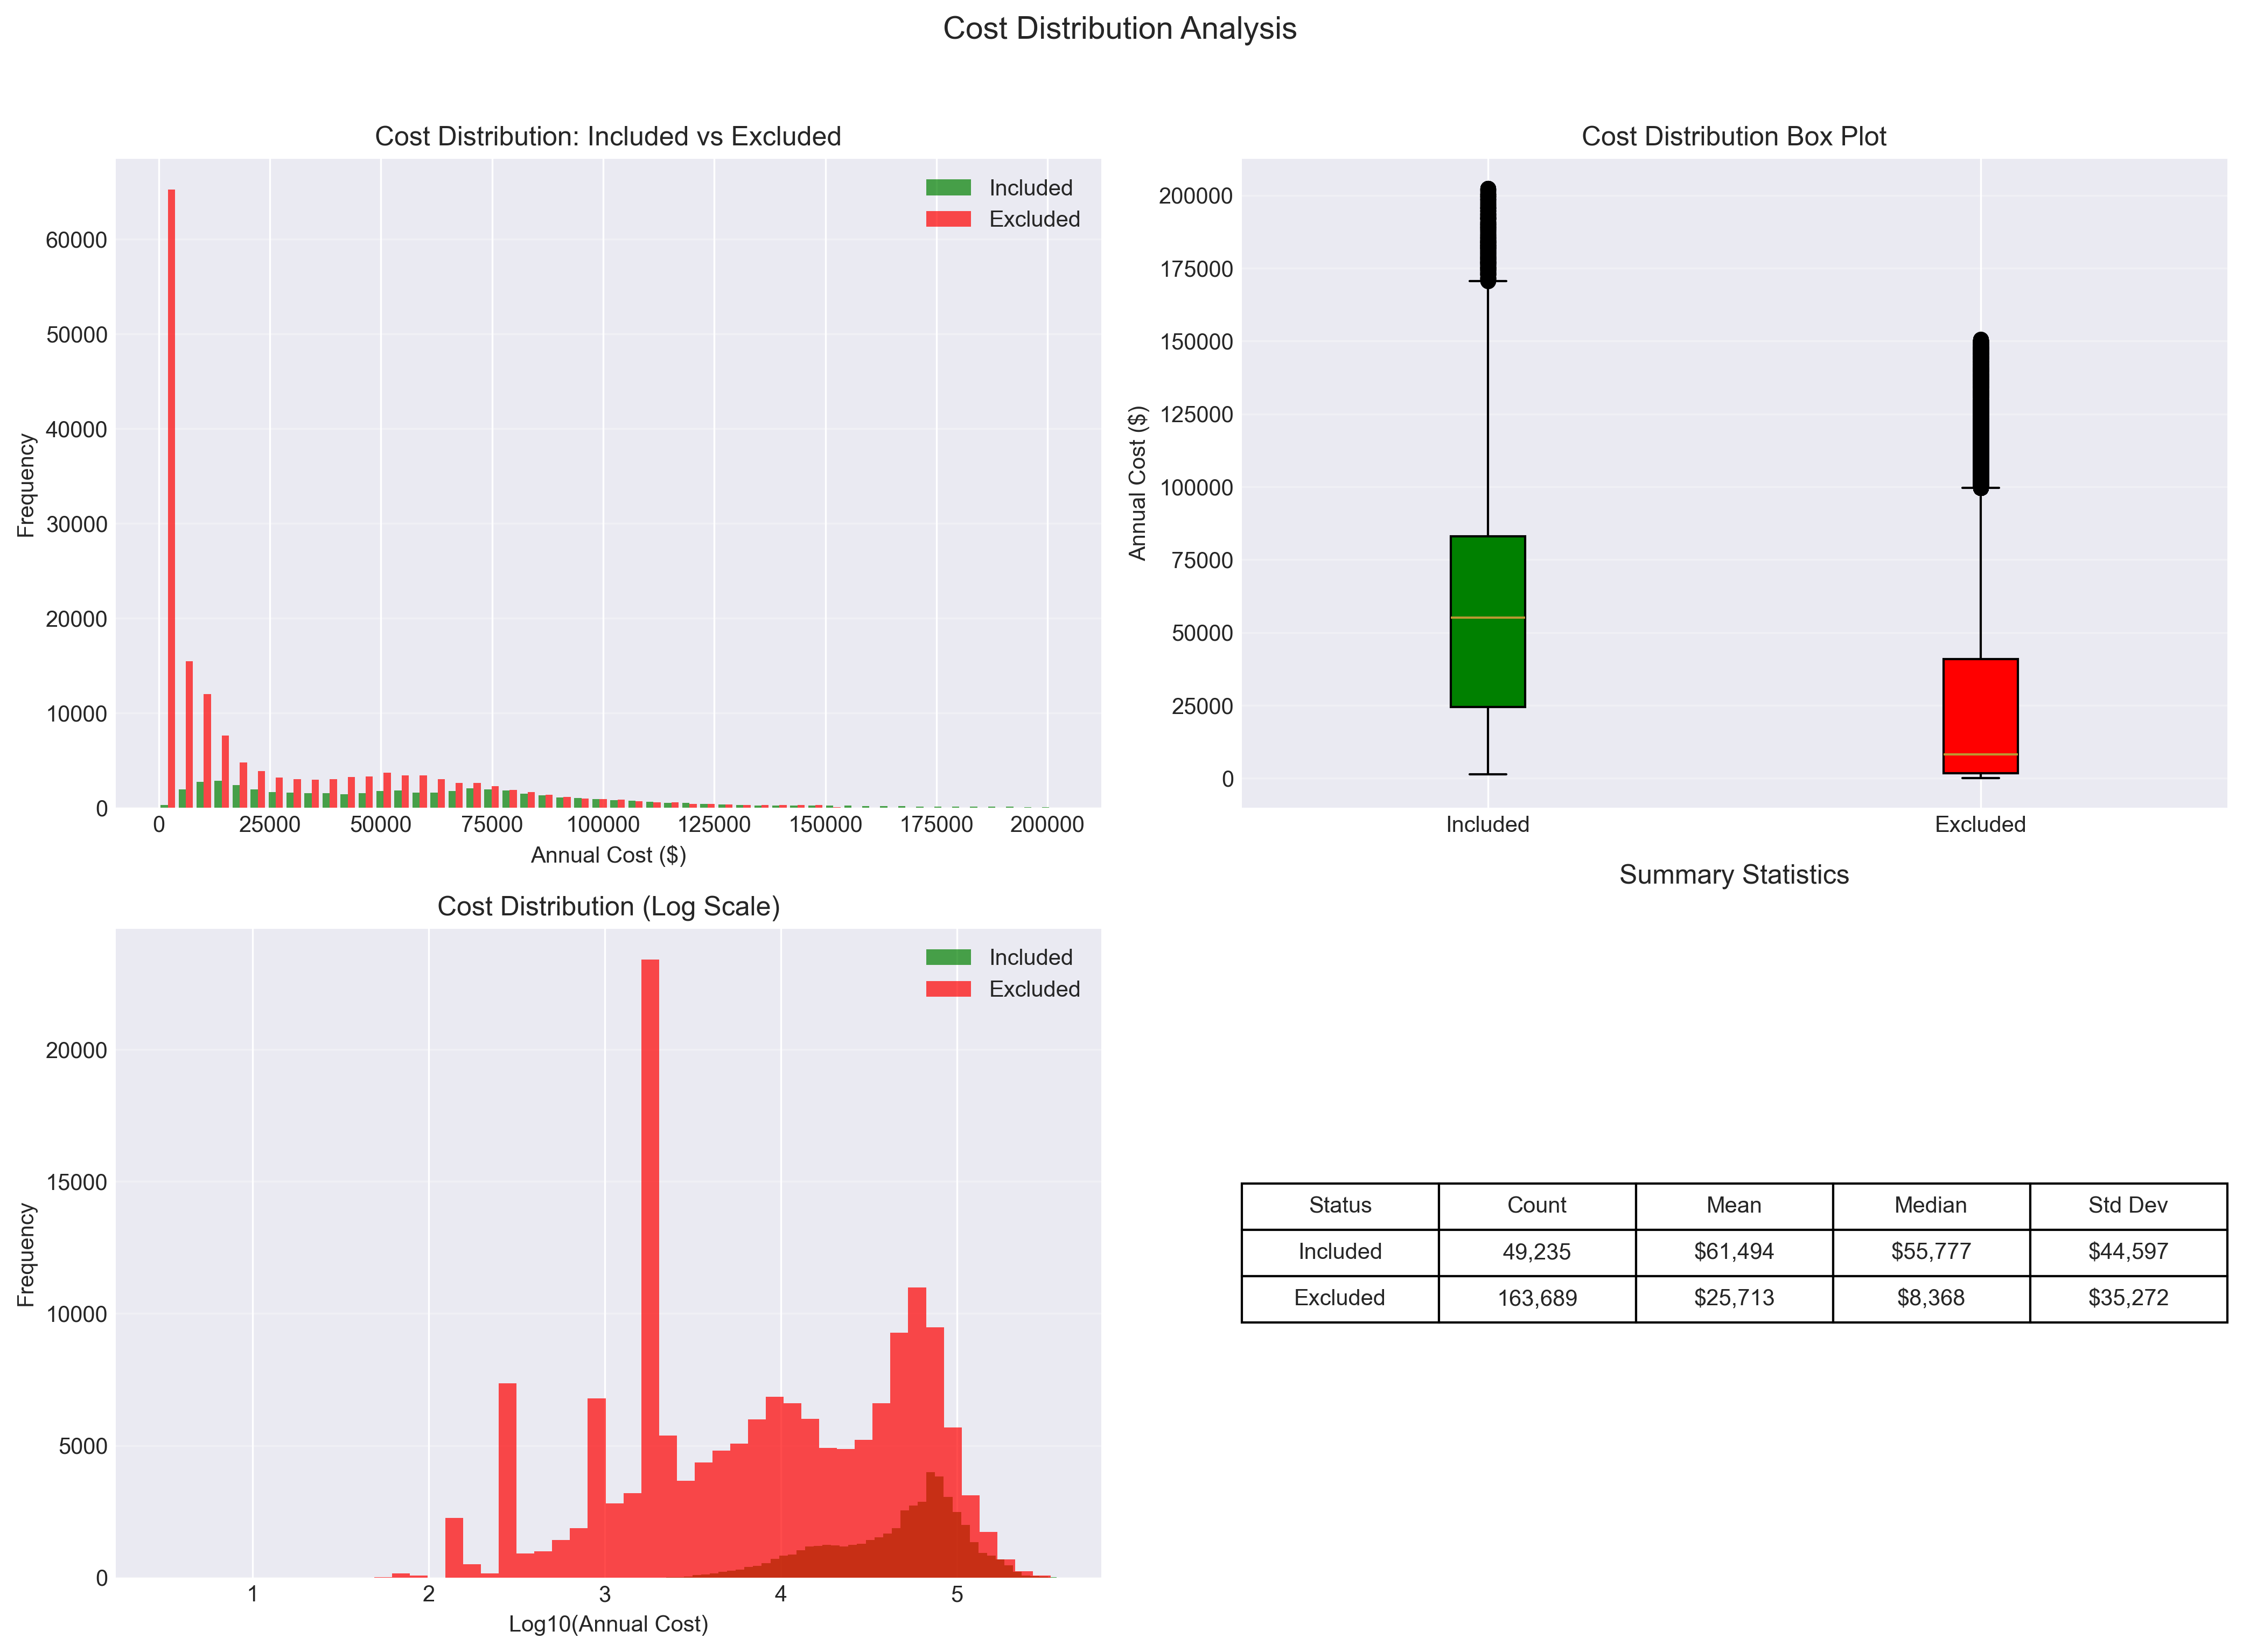
\includegraphics[width=\textwidth]{figures/cost_distributions.png}
    \caption{Comparison of cost distributions between included and excluded customer-years}
    \label{fig:cost_distributions}
\end{figure}

Figure~\ref{fig:cost_distributions} compares cost patterns between included and excluded data:
\begin{itemize}
    \item \textbf{Top-left}: Histogram overlay showing excluded records tend toward lower costs
    \item \textbf{Top-right}: Box plots revealing excluded records have wider variance and more outliers
    \item \textbf{Bottom-left}: Log-scale distribution highlighting the heavy tail in both populations
    \item \textbf{Bottom-right}: Summary statistics confirming systematically different cost profiles
\end{itemize}

\subsection{Temporal Trends}

\begin{figure}[h]
    \centering
    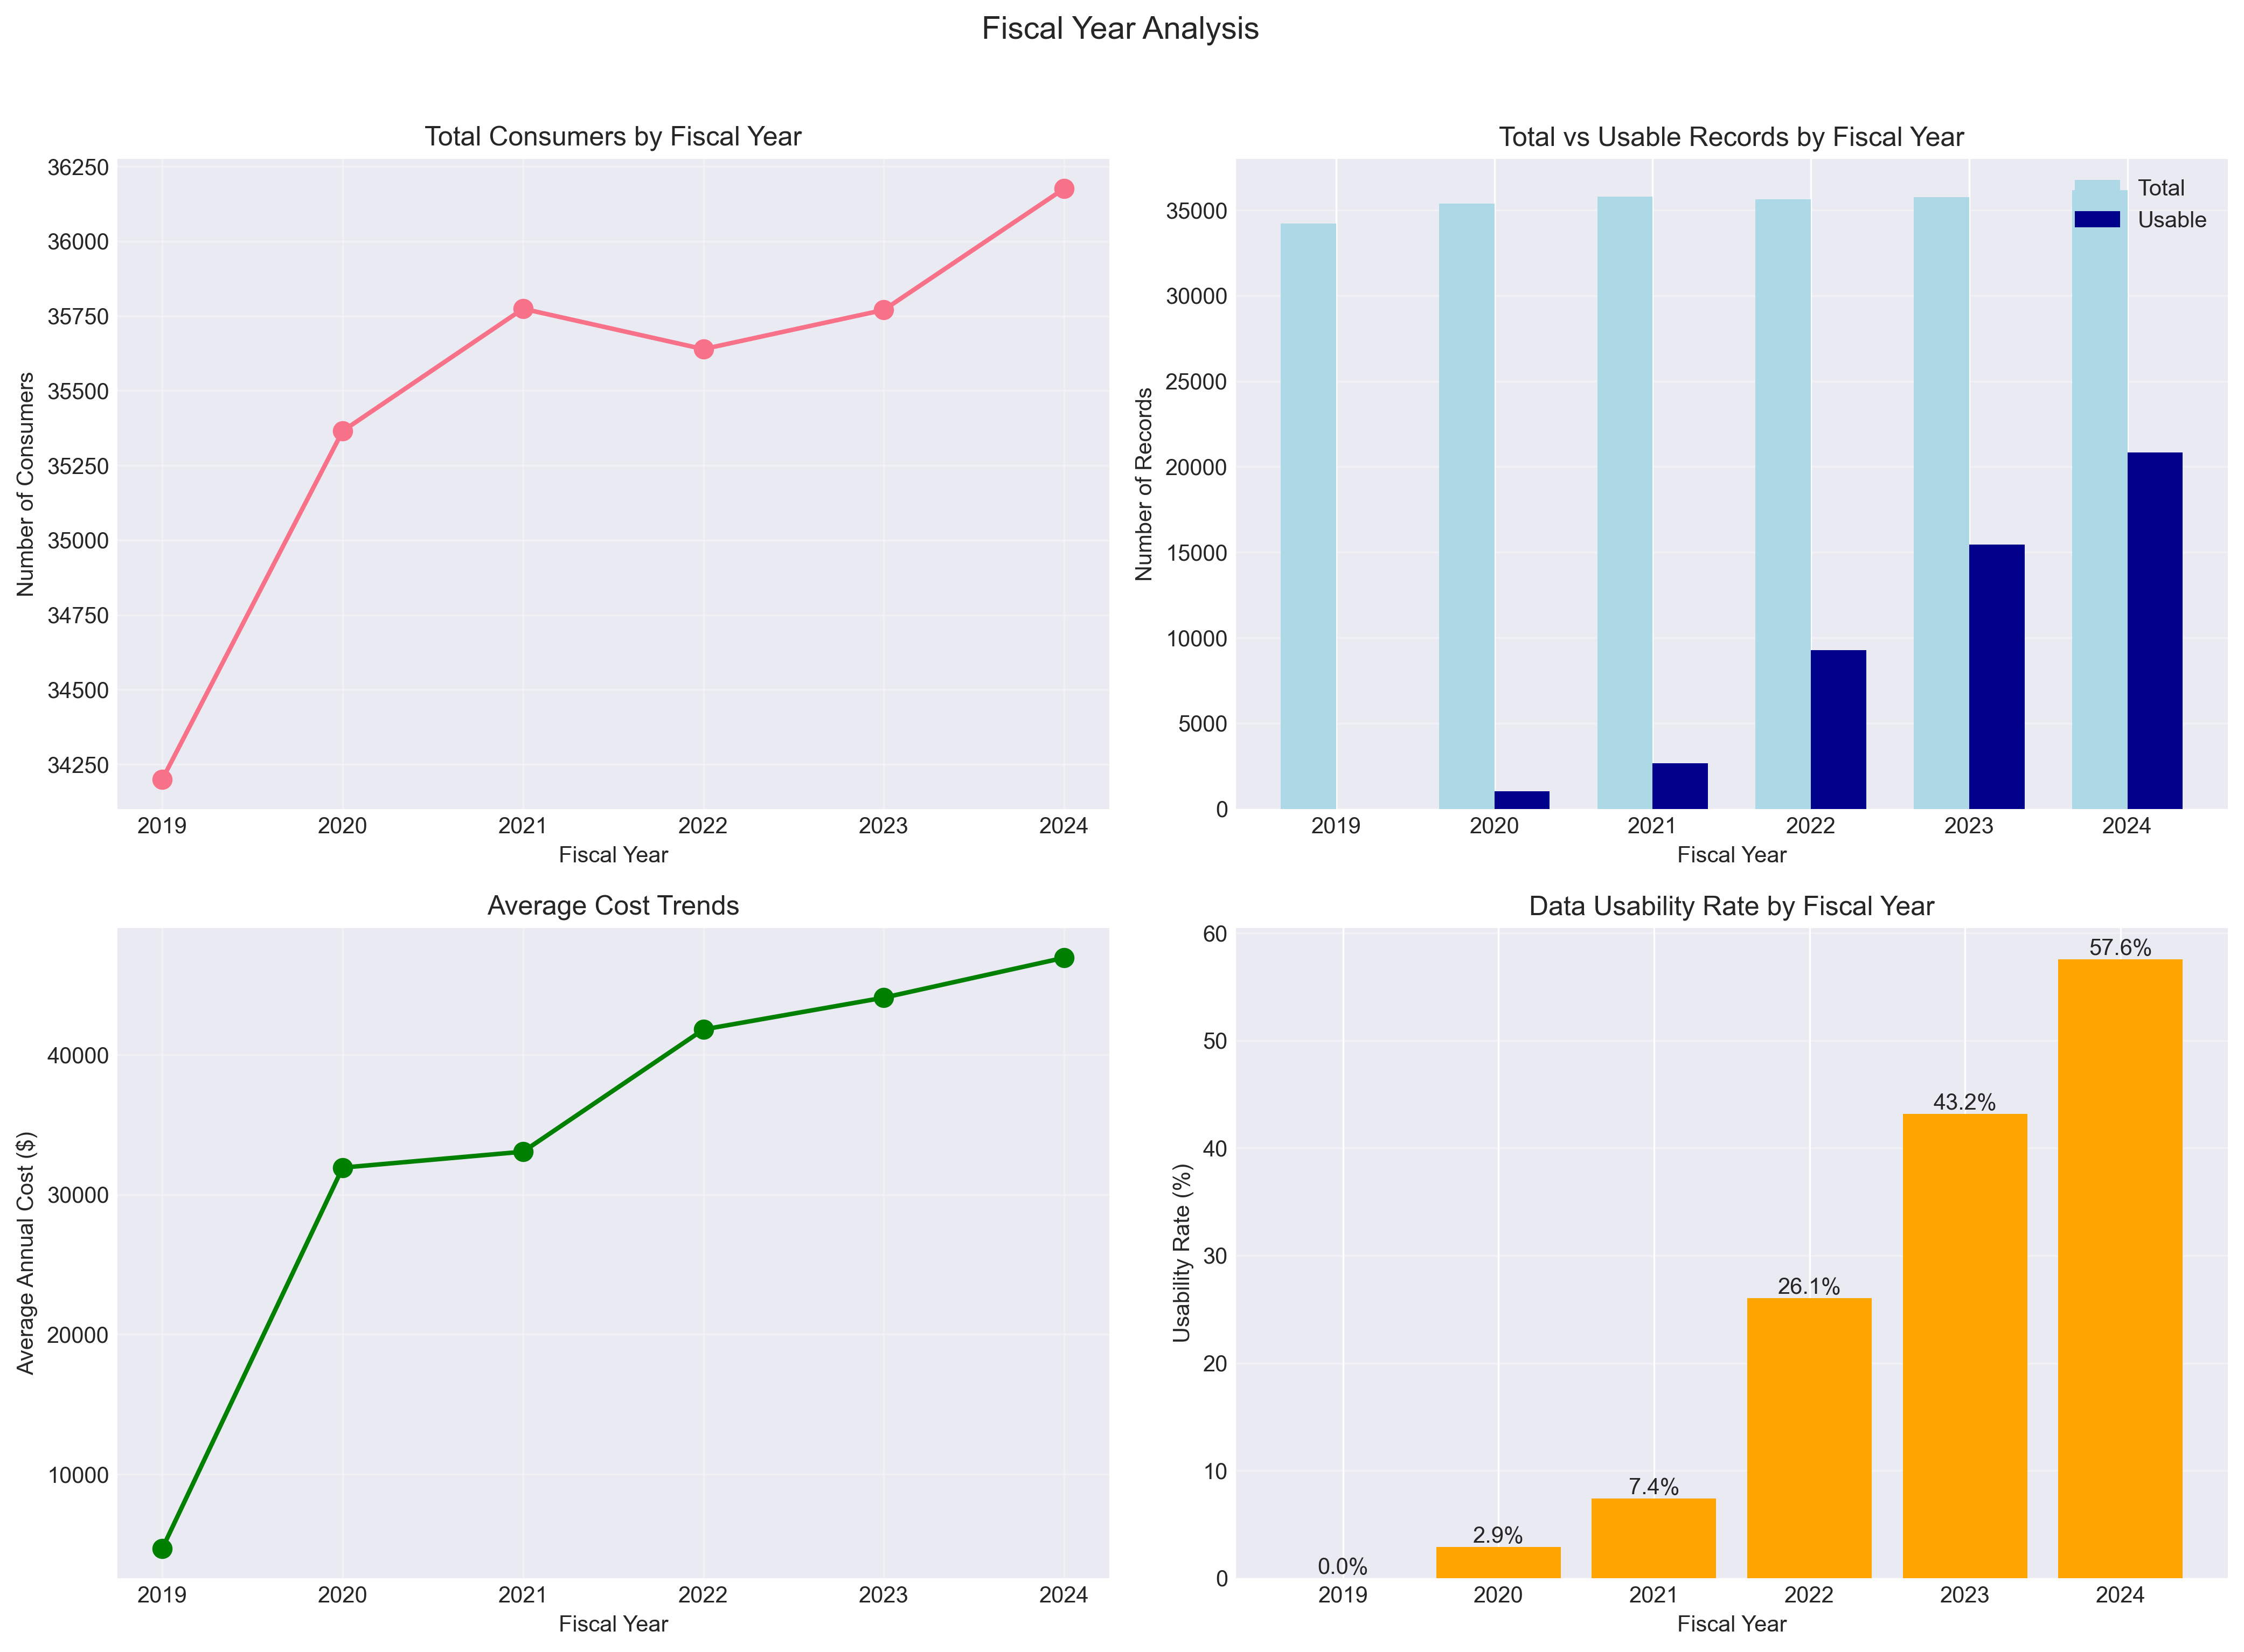
\includegraphics[width=\textwidth]{figures/fiscal_year_trends.png}
    \caption{Trends across fiscal years}
    \label{fig:fiscal_year_trends}
\end{figure}

Figure~\ref{fig:fiscal_year_trends} examines patterns over time:
\begin{itemize}
    \item \textbf{Top-left}: Customer counts by fiscal year show program growth
    \item \textbf{Top-right}: Comparison of total versus usable records reveals consistent data quality challenges
    \item \textbf{Bottom-left}: Average costs trending upward, reflecting inflation and service expansion
    \item \textbf{Bottom-right}: Data usability rates remain relatively stable across years
\end{itemize}

\subsection{Cost Outlier Analysis}

Using the Tukey method with a 3$\times$IQR threshold for extreme outliers:
\begin{itemize}
    \item Lower fence: \OutlierLowerFence
    \item Upper fence: \OutlierUpperFence
    \item Outliers below lower fence: \OutliersBelow
    \item Outliers above upper fence: \OutliersAbove
    \item Total outlier rate: \OutlierRate\%
\end{itemize}

\begin{figure}[h]
    \centering
    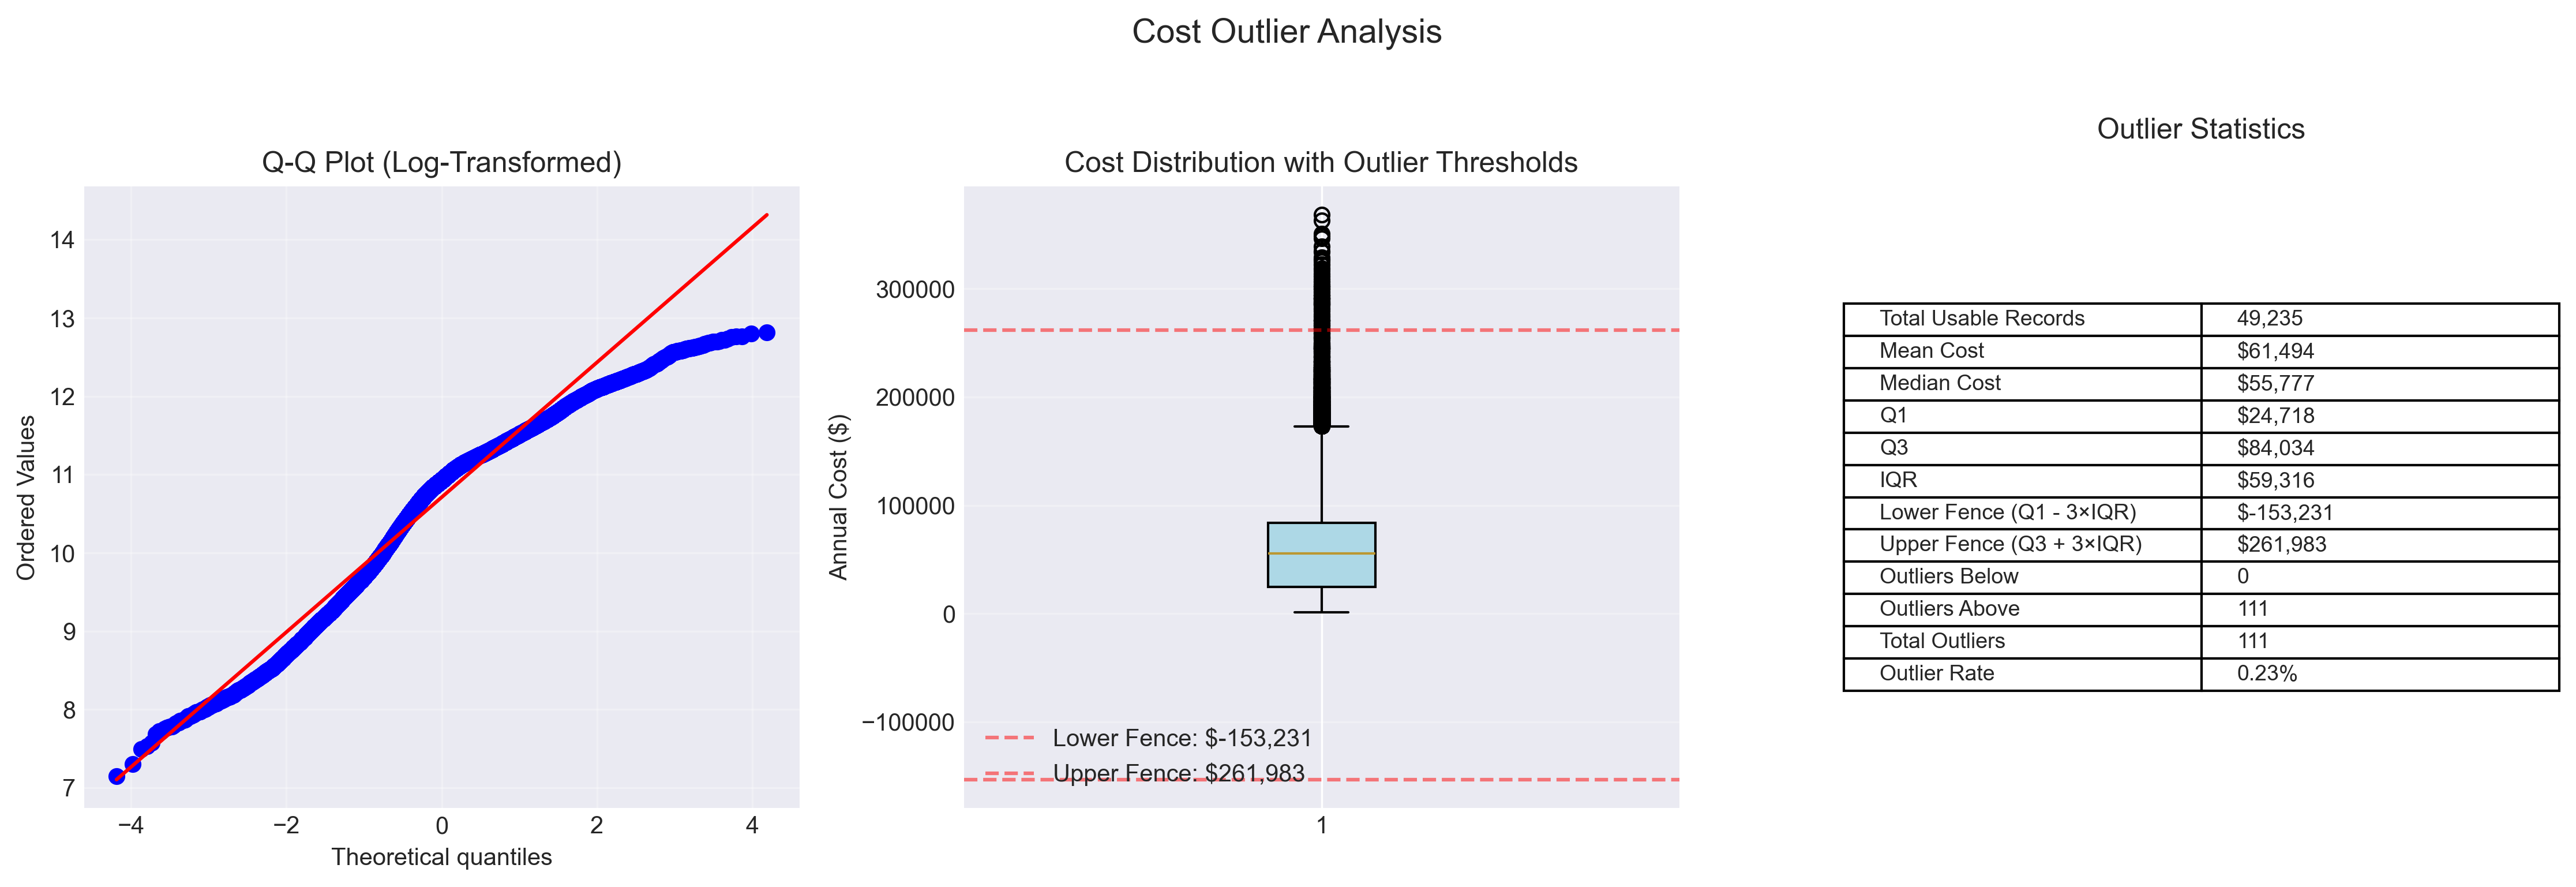
\includegraphics[width=\textwidth]{figures/cost_outliers.png}
    \caption{Cost outlier analysis}
    \label{fig:cost_outliers}
\end{figure}

Figure~\ref{fig:cost_outliers} provides outlier diagnostics:
\begin{itemize}
    \item \textbf{Left panel}: Q-Q plot of log-transformed costs shows approximate normality with heavy tails
    \item \textbf{Center panel}: Box plot with outlier thresholds (red dashed lines) identifies extreme values
    \item \textbf{Right panel}: Statistical summary quantifying outlier prevalence
\end{itemize}

\subsection{Exclusion Overlap Analysis}

\begin{figure}[h]
    \centering
    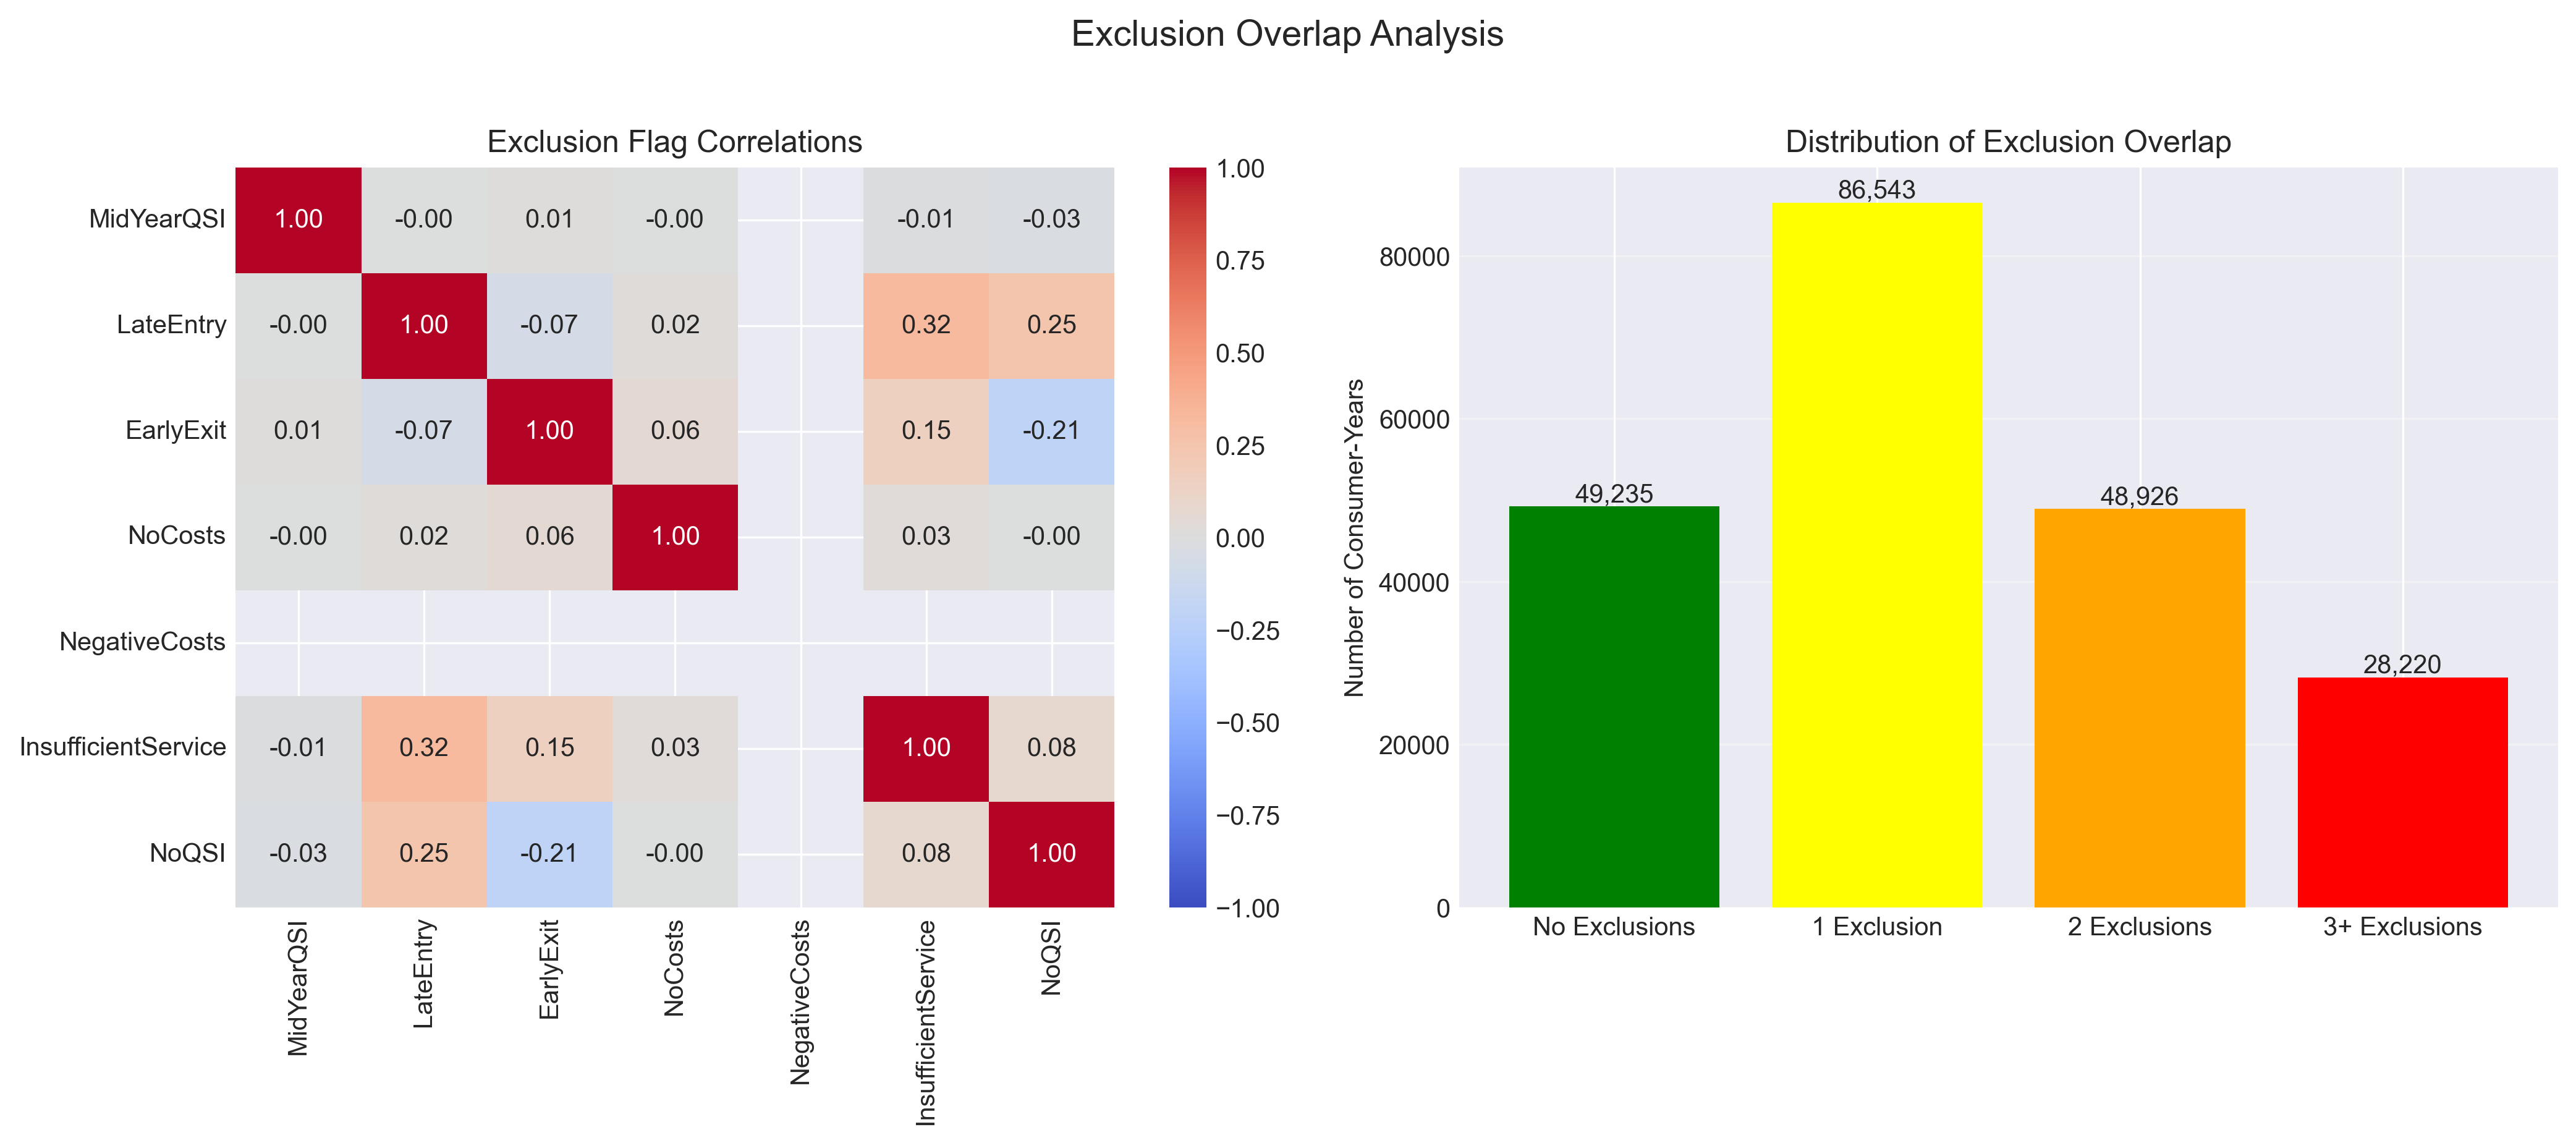
\includegraphics[width=\textwidth]{figures/exclusion_overlap.png}
    \caption{Analysis of exclusion flag correlations and overlap}
    \label{fig:exclusion_overlap}
\end{figure}

Figure~\ref{fig:exclusion_overlap} examines relationships between exclusion criteria:
\begin{itemize}
    \item \textbf{Left panel}: Correlation heatmap reveals which exclusion reasons tend to co-occur (red indicates positive correlation)
    \item \textbf{Right panel}: Bar chart showing most excluded records have multiple issues, justifying the conservative approach
\end{itemize}

\subsection{Trajectory Analysis Feasibility}

For the proposed individual trajectory modeling:
\begin{itemize}
    \item \textbf{\CustomersWithTrajectory{} customers (\PctWithTrajectory\%)} have sufficient data for individual trajectory calculation
    \item \textbf{\CustomersWithGaps{} customers (\PctWithGaps\%)} have gaps in their yearly data
    \item Customers without multi-year data will require group-based trajectory imputation
\end{itemize}

\subsection{Recommendations}

Based on this analysis:

\begin{enumerate}
    \item \textbf{Data Sufficiency}: With \CustomerPctOneYear\% of customers having usable data and \CustomerPctTwoPlusYear\% having multi-year data, the dataset supports model calibration but requires careful handling of limited trajectory coverage.
    
    \item \textbf{Trajectory Modeling}: The proposed trajectory approach is feasible for approximately \PctWithTrajectory\% of customers. The remaining customers will require cluster-based imputation.
    
    \item \textbf{Exclusion Strategy}: The conservative approach excluding customer-years with mid-year QSI changes affects \ExclusionMidYearQSIPct\% of records but ensures clean QSI-to-cost mapping.
    
    \item \textbf{Model Robustness}: Models should be tested for sensitivity to the exclusion criteria and validated on both included and excluded populations where feasible.
\end{enumerate}

% % ⚠ ======================================== ⚠ 

% \section{Data Quality and Exclusion Strategy}

% \subsection{Data Availability Assessment}

% The initial data quality analysis examined \TheTotalNumberCustomers{} unique customers in the Agency for Persons with Disabilities (APD) database, spanning fiscal years \TheInitialYear{} through \TheFinalYear{}. Each fiscal year runs from September 1 through August 31, creating potential complications when Questionnaire for Situational Information (QSI) assessments occur mid-year.

% The outlier analysis revealed substantial data quality challenges:
% \begin{itemize}
%     \item \textbf{\CustomerNumberOneYear{} customers (\CustomerPctOneYear\%)} have at least one fiscal year of usable data
%     \item \textbf{\CustomerNumberTwoPlusYear{} customers (\CustomerPctTwoPlusYear\%)} have two or more years suitable for trajectory modeling
%     \item \textbf{\CustomerNumberNoData{} customers (\CustomerPctNoData\%)} have no usable data after applying quality criteria
% \end{itemize}

% \subsection{Exclusion Criteria}

% Customer-fiscal year records are excluded from calibration if they exhibit any of the following characteristics:

% \begin{enumerate}
%     \item \textbf{Mid-year QSI changes}: Multiple QSI assessments within a single fiscal year create ambiguity in attributing costs to specific QSI scores
%     \item \textbf{Late entry}: Customers entering the system more than 30 days after fiscal year start
%     \item \textbf{Early exit}: Customers leaving the system more than 30 days before fiscal year end
%     \item \textbf{Zero or negative costs}: Records with \$0 or negative total paid amounts
%     \item \textbf{Insufficient service days}: Fewer than 30 service days within the fiscal year
%     \item \textbf{Missing QSI assessment}: No QSI assessment linked to the fiscal year
% \end{enumerate}

% This conservative approach prioritizes data quality over quantity, ensuring that model calibration uses only complete, unambiguous customer-year records.

% % ⚠ ===================================== ⚠ 
% % ⚠  DO *NOT* EDIT proration_commands.tex ⚠ 
% % ⚠  DO *NOT* EDIT proration_analysis.tex ⚠ 
% % ⚠ ===================================== ⚠ 
% % These file are produced by executing the program ProrationAnalysis.py
% % Any change in those files will be lost with every execution of the analysis pipeline 
% % Proration Analysis Statistics
% Generated: 2025-09-28 18:55:04

% Coverage statistics
\renewcommand{\ProrationFullYearPct}{70.3}
\renewcommand{\ProrationHighCoveragePct}{78.2}
\renewcommand{\ProrationMedianRFull}{754.80}
\renewcommand{\ProrationMedianRLow}{1.96}

% Customer counts
\renewcommand{\ProrationTotalCustomerYears}{212,924}
\renewcommand{\ProrationFullYearCount}{149,702}
\renewcommand{\ProrationHighCoverageCount}{166,577}

% \subsection{Proration Analysis and Decision}

Given the substantial data loss from excluding mid-year QSI changes, we investigated whether costs could be prorated for partial-year records. The analysis examined monthly cost distributions for all customers, calculating two metrics:

\begin{align}
q &= \frac{\text{months with services}}{12} \\
r &= \sum_{i=1}^{12} \frac{(m_i - \bar{m})^2}{\bar{m}}
\end{align}

where $m_i$ represents monthly expenses and $\bar{m}$ is the average monthly expense for that customer-year.

\begin{figure}[h]
    \centering
    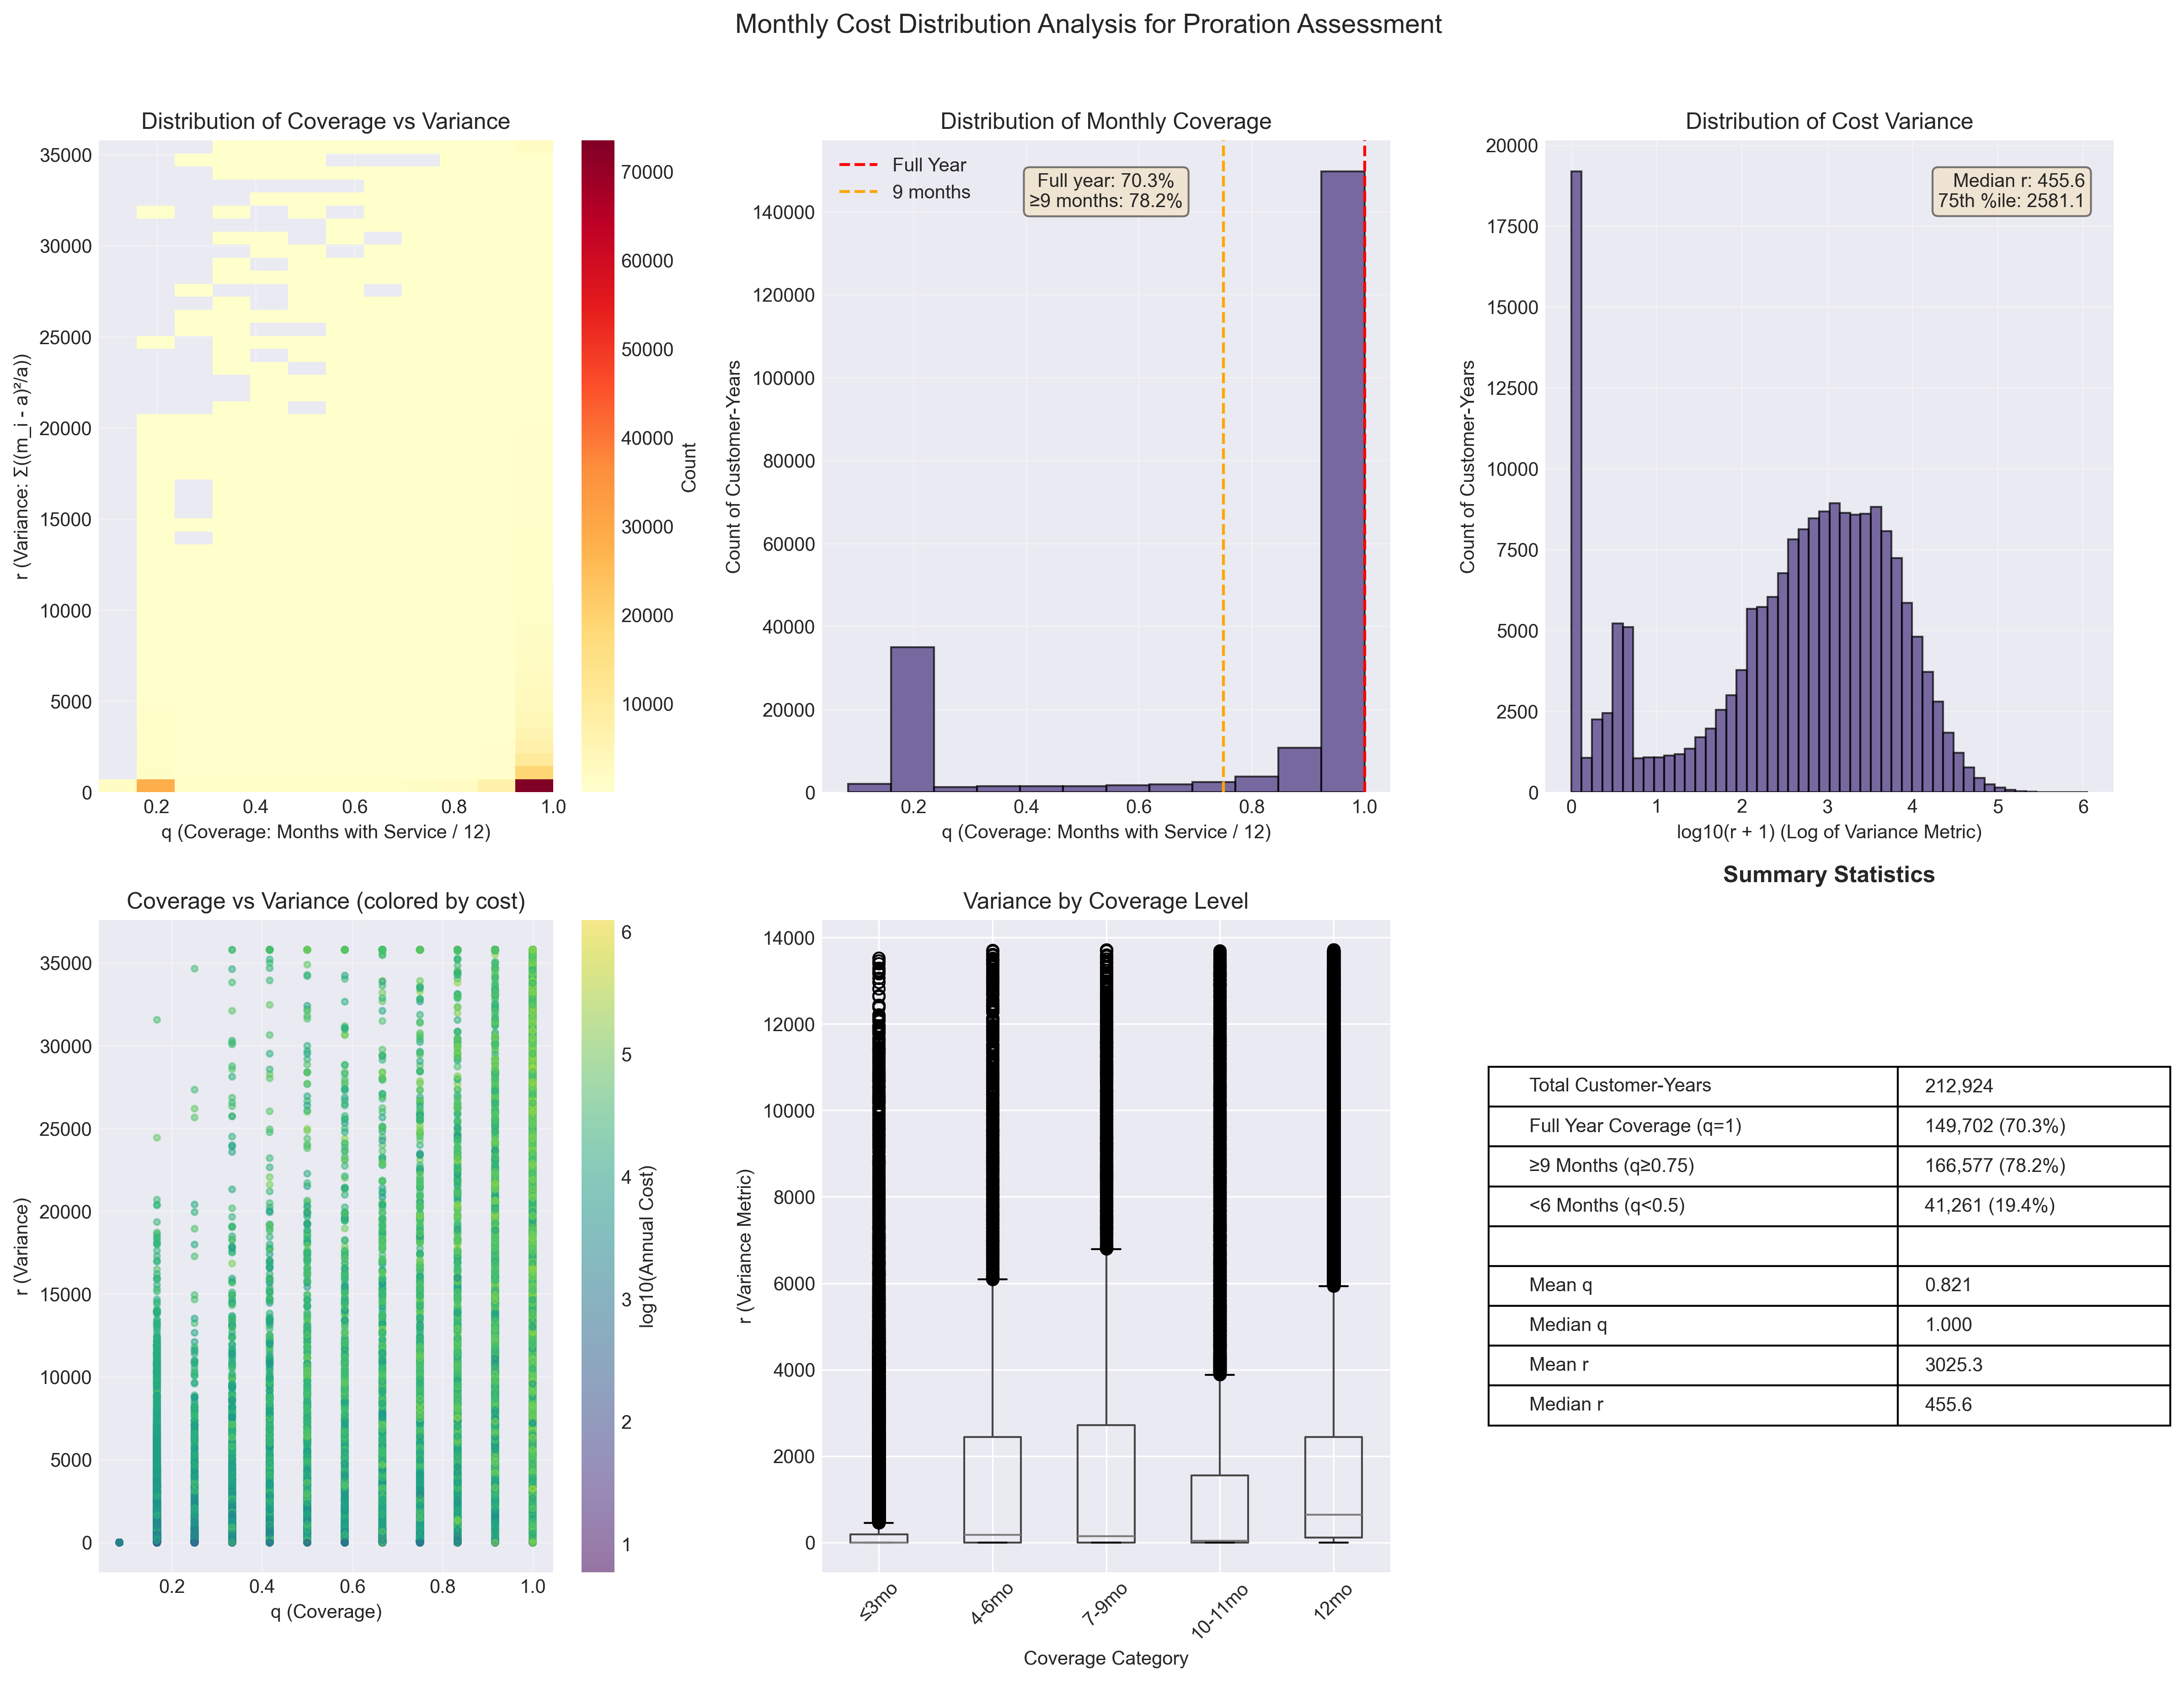
\includegraphics[width=\textwidth]{figures/cost_distribution_analysis.png}
    \caption{Monthly cost distribution analysis for proration assessment}
    \label{fig:proration_analysis}
\end{figure}

Figure~\ref{fig:proration_analysis} presents the comprehensive proration feasibility analysis:

\begin{itemize}
    \item \textbf{Top-left panel}: Two-dimensional histogram showing the relationship between coverage ($q$) and variance ($r$). The concentration of points at $q=1$ demonstrates that most customer-years have complete coverage, while the vertical spread indicates substantial variance in spending patterns.
    
    \item \textbf{Top-center panel}: Distribution of monthly coverage showing a bimodal pattern---customers either have full-year coverage or very limited engagement, with few in between.
    
    \item \textbf{Top-right panel}: Log-scale distribution of the variance metric revealing that cost variance spans multiple orders of magnitude, indicating highly heterogeneous spending patterns.
    
    \item \textbf{Bottom-left panel}: Scatter plot colored by annual cost magnitude shows that higher-cost customers tend to have more complete coverage but also higher variance.
    
    \item \textbf{Bottom-center panel}: Box plots of variance by coverage category reveal the counterintuitive finding that full-year customers have the highest cost variance.
    
    \item \textbf{Bottom-right panel}: Summary statistics quantifying the distribution patterns.
\end{itemize}

The analysis revealed critical findings:
\begin{itemize}
    \item \textbf{\ProrationFullYearPct\% of customer-years} have full 12-month coverage ($q = 1.0$)
    \item \textbf{Median variance for full-year customers}: $r = \ProrationMedianRFull$
    \item \textbf{Median variance for low-coverage customers}: $r = \ProrationMedianRLow$
\end{itemize}

The counterintuitively high variance (\ProrationMedianRFull) for full-year customers indicates highly irregular spending patterns---likely reflecting equipment purchases, hospitalizations, or seasonal service variations. This ``lumpy'' cost distribution makes proration inadvisable for several reasons:

\begin{enumerate}
    \item \textbf{Attribution ambiguity}: With such high monthly variance, costs cannot be fairly attributed to different QSI assessment periods when changes occur mid-year.
    
    \item \textbf{Systematic bias}: The inverse relationship between coverage and variance suggests partial-year customers represent a fundamentally different population that would bias model calibration.
    
    \item \textbf{Implementation complexity}: Any proration scheme would require sophisticated adjustment factors that vary by customer characteristics, introducing additional uncertainty.
\end{enumerate}

Consequently, we maintain the conservative exclusion strategy despite the data loss, as the integrity of the QSI-to-cost relationship is paramount for regulatory compliance and fair budget allocation.

% % ⚠ ===================================== ⚠ 

% \section{Modeling Framework Architecture}

% \subsection{Two-Track Trajectory Modeling}

% Given that only \CustomerPctTwoPlusYear\% of customers have sufficient multi-year data for individual trajectory calculation, we implement a dual-track approach:

% \subsubsection{Track A: Individual Trajectories}
% For the \CustomerNumberTwoPlusYear{} customers with two or more years of usable data:
% \begin{enumerate}
%     \item Calculate individual linear cost trajectories using ordinary least squares
%     \item Store intercept, slope, $R^2$, and years used for each customer
%     \item Apply trajectory: $\text{Cost}_{t+k} = \text{Base}_t + k \times \text{Slope}_i$
% \end{enumerate}

% \subsubsection{Track B: Cluster-Based Trajectories}
% For the remaining customers with single-year data:
% \begin{enumerate}
%     \item Perform K-means clustering on standardized QSI variables and demographics
%     \item Assign each customer to their nearest cluster centroid
%     \item Inherit the average slope from Track A customers within the same cluster
%     \item If cluster contains fewer than 10 Track A customers, use broader grouping
% \end{enumerate}

% \subsection{Model Calibration Pipeline}

% Each of the ten alternative models follows a standardized calibration process:

% \begin{enumerate}
%     \item \textbf{Feature Preparation}: Apply model-specific transformations and feature engineering
%     \item \textbf{Outlier Removal}: Implement model-specific outlier detection (0-10\% removal)
%     \item \textbf{Model Fitting}: Train on 80\% of data, stratified by living setting
%     \item \textbf{Cross-Validation}: Perform 10-fold stratified cross-validation
%     \item \textbf{Trajectory Integration}: Combine base predictions with trajectory adjustments
%     \item \textbf{Validation}: Evaluate on 20\% holdout test set
% \end{enumerate}

% \subsection{Master Pipeline Architecture}

% The entire framework operates through a single master script (\texttt{main\_pipeline.py}) that orchestrates all components:

% \begin{figure}[h]
% \centering
% \begin{tikzpicture}[node distance=1.5cm, auto]
%     % Define styles
%     \tikzstyle{process} = [rectangle, draw, text width=4cm, text centered, minimum height=0.8cm, fill=blue!10]
%     \tikzstyle{data} = [rectangle, rounded corners, draw, text width=3cm, text centered, fill=green!10]
%     \tikzstyle{arrow} = [thick,->,>=stealth]
    
%     % Nodes
%     \node [data] (raw) {Raw Claims \& QSI Data};
%     \node [process, below of=raw] (quality) {Data Quality Analysis};
%     \node [process, below of=quality] (proration) {Proration Feasibility};
%     \node [process, below of=proration] (prep) {Data Preparation};
%     \node [process, below of=prep] (trajectory) {Trajectory Calculation};
%     \node [process, below of=trajectory] (models) {Model Calibration (×10)};
%     \node [process, below of=models] (compare) {Comparison Analysis};
%     \node [data, below of=compare] (report) {LaTeX Report};
    
%     % Arrows
%     \draw [arrow] (raw) -- (quality);
%     \draw [arrow] (quality) -- (proration);
%     \draw [arrow] (proration) -- (prep);
%     \draw [arrow] (prep) -- (trajectory);
%     \draw [arrow] (trajectory) -- (models);
%     \draw [arrow] (models) -- (compare);
%     \draw [arrow] (compare) -- (report);
% \end{tikzpicture}
% \caption{Master pipeline architecture showing sequential processing stages}
% \end{figure}

% \section{Individual Model Specifications}

% \subsection{Model Portfolio}

% The framework evaluates ten alternative models, each with distinct theoretical foundations and assumptions:

% \begin{enumerate}
%     \item \textbf{Current Algorithm Updated}: Square-root transformation with outlier removal
%     \item \textbf{GLM-Gamma}: Generalized linear model with gamma distribution and log link
%     \item \textbf{Robust Linear Regression}: Huber regression resistant to outliers
%     \item \textbf{Weighted Least Squares}: Heteroscedasticity correction through variance weighting
%     \item \textbf{Ridge Regression}: L2-regularized regression for multicollinearity
%     \item \textbf{Log-Normal}: Linear regression with logarithmic transformation
%     \item \textbf{Quantile Regression}: Median-based estimation robust to outliers
%     \item \textbf{Bayesian Linear}: Uncertainty quantification through posterior distributions
%     \item \textbf{Principal Component Regression}: Dimensionality reduction before regression
%     \item \textbf{Deep Learning Network}: Multi-layer neural network for non-linear patterns
% \end{enumerate}

% \subsection{Common Features}

% All models utilize a consistent set of input features:
% \begin{itemize}
%     \item \textbf{Demographics}: Age groups (0-20, 21-30, 31+)
%     \item \textbf{Living Settings}: Family home, independent/supported living, residential homes (1-4)
%     \item \textbf{QSI Variables}: Q16, Q18, Q20, Q21, Q23, Q28, Q33, Q34, Q36, Q43
%     \item \textbf{Sum Scores}: BSum, FHFSum, SLFSum, SLBSum
%     \item \textbf{Temporal}: Fiscal year as numeric feature
% \end{itemize}

% \section{Validation Strategy}

% \subsection{Dual Validation Approach}

% Models undergo two complementary validation strategies:

% \subsubsection{Temporal Validation}
% \begin{itemize}
%     \item Training: Fiscal years 2018-2022
%     \item Testing: Fiscal years 2023-2024
%     \item Metrics: Year-ahead prediction accuracy
% \end{itemize}

% \subsubsection{Cross-Sectional Validation}
% \begin{itemize}
%     \item 80/20 train-test split stratified by living setting
%     \item 10-fold cross-validation on training set
%     \item Bootstrap confidence intervals (100 iterations)
% \end{itemize}

% \subsection{Performance Metrics}

% Each model is evaluated using comprehensive metrics:
% \begin{itemize}
%     \item \textbf{Regression accuracy}: $R^2$, adjusted $R^2$, RMSE, MAE, MAPE
%     \item \textbf{Model selection}: AIC, BIC
%     \item \textbf{Robustness}: Performance by demographic subgroups
%     \item \textbf{Trajectory accuracy}: Multi-year prediction errors
%     \item \textbf{Fairness}: Disparate impact analysis across protected classes
% \end{itemize}

% \section{Reproducibility and Quality Assurance}

% \subsection{Configuration Management}

% All parameters are externalized in JSON configuration files:
% \begin{itemize}
%     \item \texttt{master\_config.json}: Global settings, paths, and thresholds
%     \item \texttt{model\_configs/}: Individual model hyperparameters
%     \item Version control through Git ensures configuration tracking
% \end{itemize}

% \subsection{Reproducibility Features}

% \begin{enumerate}
%     \item \textbf{Random seed control}: Fixed seed (42) for all stochastic operations
%     \item \textbf{Checkpoint system}: Intermediate results saved for debugging/restart
%     \item \textbf{Comprehensive logging}: Detailed logs at each pipeline stage
%     \item \textbf{Data versioning}: MD5 checksums for input data files
%     \item \textbf{Environment specification}: Docker container for consistent execution
% \end{enumerate}

% \subsection{Quality Checks}

% Automated quality checks ensure data and model integrity:
% \begin{itemize}
%     \item Verification that excluded records match documented criteria
%     \item Comparison of model coefficients against expected ranges
%     \item Detection of data leakage between train and test sets
%     \item Validation of LaTeX output compilation
%     \item Performance regression tests against baseline metrics
% \end{itemize}


% \section{References}

% \begin{itemize}
%     \item Huber, P. J. (1964). Robust estimation of a location parameter. \textit{The Annals of Mathematical Statistics}, 35(1), 73--101.
%     \item Rousseeuw, P. J., \& Leroy, A. M. (2003). \textit{Robust regression and outlier detection}. John Wiley \& Sons.
%     % \item ... a dozen more...
%     \item Maronna, R., Martin, D., \& Yohai, V. (2006). \textit{Robust statistics: Theory and methods}. John Wiley \& Sons.
%     \item Florida House Bill 1103 (2024). Transparency in developmental disability services.
%     \item Tao, Y., \& Niu, X. (2015). Florida iBudget Algorithm Final Report. Florida State University.
% \end{itemize}